%
% analysis, example programs
%

\chapter{Results}
\label{ch:results}

\epigraph{Logic merely enables one to be wrong with authority.}%
{\textsc{---the doctor}} %\\\textit{The Wheel in Space}}

% \epigraph{Dionysus [is] the Master of Illusions, who could make a vine grow out
% of a ship's plank, and in general enable his votaries to see the world as the
% world's not.}%
% {\textsc{---e.\ r.\ dodds}\\\textit{The Greeks and the Irrational}}

% \epigraph{If the immutable appears recast, then you yourself have been
% transformed.}%
% {\textsc{---r.\ scott bakker}\\\textit{The Judging Eye}}


The previous chapters discussed the design, implementation and optimisation of
the Accelerate language and CUDA backend.%
\footnote{Version 0.15 release candidate: \texttt{de156af5f6d839bc6e0597d33a7a151f0e492a66}}
This chapter analyses the performance of the implementation. Benchmarks were
conducted on a single Tesla T10 processor (compute capability 1.3, 30
multiprocessors = 240 cores at 1.3GHz, 4GB RAM) backed by two quad core Xeon
E5405 CPUs (64-bit, 2GHz, 8GB RAM) running GNU/Linux (Ubuntu 12.04 LTS).
Measurements are the average of 100 runs. Programs are compiled with
ghc-7.8.2,%
\footnote{Including fix for stable name bug \#9078: \url{https://ghc.haskell.org/trac/ghc/ticket/9078}}
CUDA 6.0, gcc-4.6.3 and llvm-3.4. Parallel CPU programs are run on all eight
cores.

Haskell programs are compiled with the following options, which is the
recommended set to use when compiling Repa programs:
%
\begin{lstlisting}
-Wall -threaded -rtsopts -fllvm -optlo-O3 -Odph -fno-liberate-case
-funfolding-use-threshold100 -funfolding-keeness-factor100
\end{lstlisting}
%
CUDA programs are compiled with the options:
%
\begin{lstlisting}
-O3 -m64 -arch=sm_13
\end{lstlisting}
%
A summary of the benchmark results is shown in
Table~\ref{tab:benchmark-summary}.

\begin{table}
\centering
\begin{tabu}{llrrrrrr}
\toprule
\small
                &
                & \multicolumn{2}{c}{Contender}
                & \multicolumn{2}{c}{Accelerate}
                & \multicolumn{2}{c}{Accelerate}
                \\

\textbf{Benchmark}
                & Input size
                & \multicolumn{2}{c}{(ms)}
                & \multicolumn{2}{c}{(ms)}
                & \multicolumn{2}{c}{no optim.\ (ms)}
                \\
\midrule

Dot product     & 20M
                & 1.88 & (CUBLAS)
                & 2.34 & (124\%)
                & 4.31 & (230\%)
                \\

Black-Scholes   & 20M
                & 6.69  & (CUDA)
                & 6.19  & (92.5\%)
                & 115.6 & (1727\%)
                \\

Mandelbrot      & 2M
                & 4.99  & (CUDA)
                & 7.61  & (153\%)
                & 430.8 & (8632\%)
                \\

N-body          & 32k
                & 54.4  & (CUDA)
                & 102.9 & (189\%)
                & \multicolumn{2}{c}{\emph{(out of memory)}}
                \\

SMVM (protein)  & 2M
                & 1.05 & (CUSP)
                & 0.58 & (54.8\%)
                & 1.13 & (107\%)
                \\

Canny           & 16M
                & 46.0 & (OpenCV)
                & 100  & (217\%)
                % & \multicolumn{2}{c}{\emph{(not supported)}}
                & 105  & (227\%)
                \\

Fluid flow      & 2M
                & 974.4 & (Repa)
                & 208.5 & (21.4\%)
                & 220.9 & (22.7\%)
                \\

Radix sort      & 2M
                & 404   & (Nikola)
                & 221.5 & (54.8\%)
                & 283.3 & (70.1\%)
                \\

Floyd-Warshall  & 1k
                & 7766 & (Repa)
                & 836  & (10.8\%)
                % & \multicolumn{2}{c}{\emph{(timeout)}}
                & 840  & (10.8\%)
                \\

MD5             & 1M
                & 1.29 & (Hashcat)
                & 3.80 & (294\%)
                & \multicolumn{2}{c}{\emph{(error)}}
                \\

K-Means         & 100k
                & 24.7 & (MonadPar)
                & 1.01 & (4.1\%)
                & 0.77 & (3.1\%)
                \\

Ray tracer      & 16M
                & 2027 & (Repa)
                & 2174 & (107\%)
                & \multicolumn{2}{c}{\emph{(error)}}
                \\

LULESH          & 91k
                & 1.11 & (CUDA)
                & 2.09 & (189\%)
                & \multicolumn{2}{c}{\emph{(error)}}
                \\
\bottomrule
\end{tabu}
\caption[Benchmark summary]{Summary of the performance of the benchmark
    programs, before and after optimisations. Note that array-level sharing
    recovery is always enabled, otherwise most programs simply do not run in a
    reasonable amount of time. The MD5, Ray tracer, and LULESH programs also
    fail to run without scalar sharing recovery.}
\label{tab:benchmark-summary}
\end{table}


\section{Runtime overheads}

Runtime program optimisation, code generation, kernel loading, data transfer,
and so on can contribute significant overhead to short lived GPU computations.
Accelerate mitigates these overheads via caching and memoisation. For example,
the first time a particular expression is executed it is compiled to CUDA code,
which is reused for subsequent invocations. This section analyses those
overheads, so that they can be factored out later when we discuss the effects of
the program optimisations on kernel runtimes of the benchmark programs.


\subsection{Program optimisation}

The Floyd-Warshall algorithm for finding the shortest paths in a directed graph,
discussed in Section~\ref{sec:floyd_warshall}, was found to cause serious
problems with the original implementation of the optimisations discussed in this
thesis. Thus, changes were made to ensure that the complexity of the
optimisations is not exponential in the number of terms in the program. In
particular, the reified program consists of a sequence of let bindings to
producer operations, so the handling of let bindings
(\S\ref{sec:binder_elimination}) and the representation of producers that
separates the delayed array representation from the captured environment terms
(\S\ref{sec:representing_producers}) was found to be crucial.
Figure~\ref{fig:convertAcc} shows the time to optimise the Floyd-Warshall
program with and without these changes of the optimisation pipeline.

\begin{figure}
    \begin{center}
        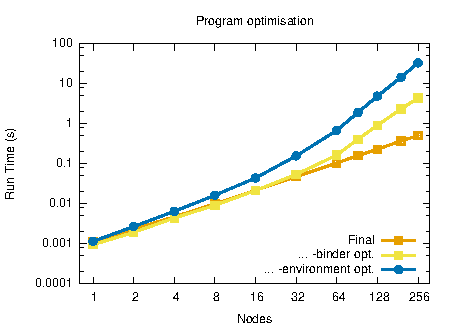
\includegraphics[width=0.8\textwidth]{images/results/convertAcc/convertAcc}
    \end{center}
    \caption[Program optimisation runtimes]{Time to optimise the Floyd-Warshall
        program, comparing the final version of the fusion algorithm to earlier
        implementations which exhibit exponential scaling in the number of AST
        terms. Note the log-log scale.}
    \label{fig:convertAcc}
\end{figure}

\subsection{Memory management \& data transfer}

Figure~\ref{fig:data_transfer} shows the time to transfer data to and from the
device. Observe that the data transfer time can account for a significant
portion of the overall execution time for some benchmarks.
% The measured times allow the Accelerate runtime system to avoid allocating data
% on every transfer to the device.

% tk: importance of using weak pointers, so data transfers ``escape'' the black
%     box of evaluating the AST --> hashcat.
% tk: importance of the nursery for reducing calls to malloc/free

\begin{figure}
    \centering
    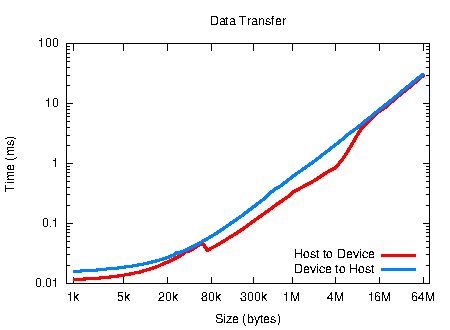
\includegraphics[width=0.8\textwidth]{images/results/bandwidth/time} \\
    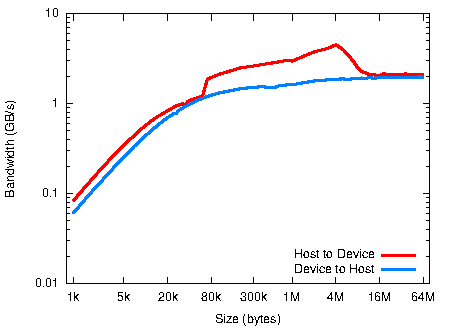
\includegraphics[width=0.8\textwidth]{images/results/bandwidth/bandwidth}
    \caption{Data transfer time and bandwidth measurements}
    \label{fig:data_transfer}
\end{figure}

\subsection{Code generation \& compilation}

To demonstrate the effectiveness of our persistent kernel caching techniques
(\S\ref{sec:caching_compiled_kernels}), Table~\ref{tab:compilation_times} lists
the code generation and compilation times for each of the benchmark programs
considered in this chapter. Compilation times are measured by compiling the
generated code directly with the @nvcc@ command line tool. Times are the average
of 10 evaluations. In contrast, loading the pre-compiled kernels from the
on-disk cache typically takes less than one millisecond.

\begin{table}
    \centering
    \begin{tabu}{lrrrr}
\toprule
\small

\textbf{Benchmark}
    & \multicolumn{1}{c}{No. kernels}
    & \multicolumn{1}{c}{Generation (ms)}
    & \multicolumn{1}{c}{Compilation (s)}
    \\
    \midrule

Dot Product
    & 2
    & 1.03      % 1.029109 ms
    & 1.97 (3.87)
    \\

Black-Scholes
    & 1
    & 0.59      % 590.6926 µs
    & 1.95 (1.95)
    \\

Mandelbrot
    & 1
    & 0.65      % 653.9279 µs
    & 1.94 (1.94)
    \\

N-Body
    & 2
    & 1.47      % 474.0642 µs + 994.1904 µs
    & 1.99 (3.88)
    \\

SMVM
    & 4
    & 4.84      % 2.014550 ms + 822.1717µs
    & 2.01 (7.82)
    \\

Canny
    & 11
    & 5.91      % 220.2916µs + 618.6954µs + 682.8163µs + 1.223156ms + 573.1638µs + 126.0751µs + 2.065717ms + 77.02148µs + 320.2738µs
    & 4.91 (21.4)
    \\

Fluid flow
    & 11
    & 10.47     % 171.6616µs + 175.5634µs + 410.1354µs + 939.1292µs + 2.523173ms + 3.000089ms + 1.566233ms + 347.7783µs + 1.139579ms
    & 5.07 (21.6)
    \\

Radix sort
    & 8
    & 5.21      % 220.7054 µs + 2.324179 ms + 2.314650 ms + 349.0219 µs
    & 2.49 (15.6)
    \\

Floyd-Warshall
    & 2
    & 0.51      % 254.0066 µs + 254.5462 µs
    & 1.96 (3.85)
    \\

Hashcat
    & 1
    & 11.60     % 11.59957
    & 2.31 (2.31)
    \\

K-Means
    & 5
    & 7.33      % 1.619417 ms + 2.749049 ms + 208.3831 µs + 2.749397 ms
    & 2.18 (10.0)
    \\

Ray
    & 1
    & 40.11     % 40.10992
    & 3.73 (3.73)
    \\

LULESH
    & 28
    & 118.3     % 172.7553 µs + 67.50892 ms + 6.286733 ms + 620.4056 µs + 17.19437 ms + 9.231346 ms + 5.073148 ms + 2.529079 ms + 198.7472 µs + 204.6181 µs + 205.3183 µs + 293.0012 µs + 204.4255 µs + 1.913622 ms + 2.501033 ms + 814.0013 µs + 143.9810 µs + 143.0060 µs + 132.4113 µs + 150.3967 µs + 1.794947 ms + 128.4771 µs + 268.0296 µs + 149.0522 µs + 282.7501 µs + 130.2992 µs
    & 12.6 (71.4)
    \\

\bottomrule

    \end{tabu}
    \caption[Benchmark code generation and compilation times]{Code generation
        and compilation times for the benchmark programs. Kernels are compiled
        concurrently, one per core, as is done by the Accelerate runtime system.
        The equivalent sequential compilation time is shown in parenthesis.}
    \label{tab:compilation_times}
\end{table}

% tk: measure \& tabulate some code generation / compilation times
% tk: persistent cache, perhaps just a mention?


\section{Dot product}
\label{sec:dotp}

Dot product, or scalar product, is an algebraic operation that takes two
equal-length sequences of numbers and returns a single number by computing the
sum of the products of the corresponding entries in the two sequences. Dot
product can be defined in Accelerate using the code shown in
Listing~\ref{lst:dotp}, and seen previously.

\begin{lstlisting}[style=haskell_float
    ,label=lst:dotp
    ,caption={Vector dot-product}]
dotp :: Acc (Vector Float) -> Acc (Vector Float) -> Acc (Scalar Float)
dotp xs ys = A.fold (+) 0                       -- sum result of\ldots
           $ A.zipWith (*) xs ys                -- \ldots element-wise multiplying inputs
\end{lstlisting}

Figure~\ref{fig:dotp} show the result of running this code, compared to several
other sequential and parallel implementations. The \texttt{Data.Vector} baseline
is sequential code produced by stream fusion~\cite{Coutts:2007kp}, running on
the host CPU. The \texttt{Repa} version runs in parallel on all eight cores of
the host CPU, using the fusion method of delayed arrays~\cite{Keller:2010er}.
% The \texttt{NDP2GPU}~\cite{Bergstrom:2012bi} version compiles NESL
% code~\cite{Blelloch:1995ut} down to CUDA. The performance of NDP2GPU suffers
% because it uses the legacy NESL compiler for the front-end, which introduces
% redundant administrative operations that are not strictly needed when evaluating
% a dot product.

\begin{figure}
    \begin{center}
        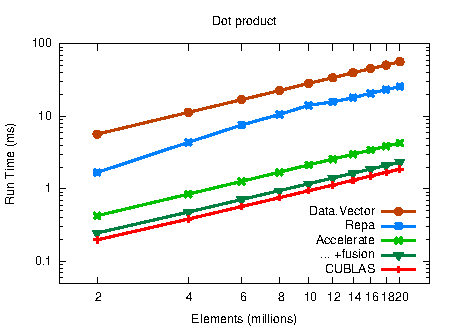
\includegraphics[width=0.8\textwidth]{images/results/dotp/dotp}
    \end{center}
    \caption[Vector dot product kernel benchmarks]{Kernel runtimes for vector
        dot product, in Accelerate with and without optimisations, compared to
        other parallel GPU and CPU implementations. Note the log-log scale.}
    \label{fig:dotp}
\end{figure}

Without optimisations the Accelerate version executes in approximately twice the
time of the CUBLAS version. Since the individual aggregate operations consist of
only a single arithmetic operation each, the problem can not be a lack of
sharing.


\subsection{Too many kernels}

The slow-down in the unoptimised version is due to Accelerate generating one GPU
kernel function for each aggregate operation in the source program. The use of
two separate kernels requires the intermediate array produced by @zipWith@ to be
constructed in GPU memory, which is then immediately read back by @fold@. In
contrast, the CUBLAS version combines these operations into a single kernel. As
this is a simple memory bound benchmark, we would expect the lack of fusion to
double the runtime, which is what we observe.

The fused version of dot product combines the aggregate computations by
embedding a function from array indices to array values of type @(sh -> a)@ into
the reduction, represented here as the second argument to the constructor
@Delayed@. This scalar function does the work of element wise multiplying the
two input vectors, and is performed on-the-fly as part of the reduction kernel
instead of requiring an intermediate array. See Section~\ref{sec:array_fusion}
for more information. Applied to two manifest arrays, the following embedded
program will be executed:

\begin{lstlisting}[style=haskell]
let a0 = use (Array ...) in                       -- manifest input arrays
let a1 = use (Array ...) in
fold (\x0 x1 -> x0 + x1) 0.0
     (Delayed (intersect (shape a0) (shape a1))   -- extent of the input array
              (\x0 -> (a0!x0) * (a1!x0)))         -- function to generate a value at each index
\end{lstlisting}

While the fused Accelerate version is $25\times$ faster than the sequential
version executed on the CPU, it is still approximately $20\%$ slower than the
hand-written CUBLAS version. As dot product is a computationally simple task,
any additional overheads in the implementation will be significant. To see why
this version is still slightly slower, we continue by analysing the generated
code to inspect it for sources of overhead.


% \subsection{Duplicate loop counters}
%
% The fused dot product operation will only perform the element wise
% multiplication of the two input arrays in the first step of the tree reduction
% (\S\ref{sec:parallel_reduction}). This occurs in the phase of the cascaded
% algorithm when individual threads sequentially sum multiple elements. After
% embedding the fused producer, the following CUDA code is generated for the inner
% loop of this step:
% %
% % pookie is the bestest
% % bubbaboo ish silly
% % kekekee
% % i can't put smiley faces in cause weird things happen
% % hehe^{this is my thesis
% % please like it
% % i worked really hard
% % and writed a lots
% % }<++>
% %
% %
% \begin{lstlisting}[style=cuda
%     ,firstnumber=18
%     ,label=lst:dotp_cuda
%     ,caption={Generated CUDA code for the first step of fused dot product}]
% for (ix += gridSize; ix < shapeSize; ix += gridSize) {
%     const Int64 v2 = ix;
%     const int v3 = toIndex(shIn0, shape(v2));
%     const int v4 = toIndex(shIn1, shape(v2));
%
%     x0 = arrIn0_a0[v3] * arrIn1_a0[v4];
%     y0 = x0 + y0;
% }
% \end{lstlisting}
% %
% We have four loop counters: @ix@, @v2@, @v3@ and @v4@ ---
% two for the source arrays and two to convert between the multidimensional and
% linear representations. These counters contain the same value and are
% incremented in lockstep. In addition to the superfluous arithmetic, the
% duplication of counters unnecessarily increases register pressure.
%
% \marginnote{this was unexpected}
% The corresponding section of PTX~\cite{NVIDIA:2012vj} code is for this loop is
% shown in Listing~\ref{lst:dotp_ptx}. To retrieve the data from the first input
% array, the input array pointer is retrieved (line~\ref{lst:dotp_ptx_ldparam}),
% the offset stored in register @rd16@ added to it
% (line~\ref{lst:dotp_ptx_add}), and then the value read from global memory at
% this address (line~\ref{lst:dotp_ptx_ldglobal}). Happily, we note that
% retrieving the second input element \emph{also} uses the offset stored in
% register @rd16@ (line~\ref{lst:dotp_ptx_ldglobal2}).
% %
%
% \begin{lstlisting}[style=ptx
%     ,float
%     ,firstnumber=103
%     ,label=lst:dotp_ptx
%     ,caption={[PTX code for the first step of fused dot product]
%         PTX code for the first step of fused dot product (sm13)}]
%  //  18          for (ix += gridSize; ix < shapeSize; ix += gridSize) {
%         cvt.u32.u16     %r10, %nctaid.x;
%         mul.lo.u32      %r11, %r10, %r1;
%         add.s32         %r12, %r11, %r7;
%         mov.s32         %r13, %r12;
%         setp.le.s32     %p2, %r8, %r12;
%         `%p2 bra        $Lt_0_13058;
%         cvt.s64.s32     %rd12, %r12;
%         cvt.s64.u32     %rd13, %r11;
% $Lt_0_14082:
%  //<loop> Loop body line 18, nesting depth: 1, estimated iterations: unknown
%         .loc    16      24      0
%  //  20              const int v3 = toIndex(shIn0, shape(v2));
%  //  21              const int v4 = toIndex(shIn1, shape(v2));
%  //  22
%  //  23              x0 = arrIn0\_a0[v3] * arrIn1\_a0[v4];
%  //  24              y0 = x0 + y0;
%         cvt.s32.s64     %rd14, %rd12;                           (@* \label{lst:dotp_ptx_cvt1} *@)
%         cvt.s32.s64     %r14, %rd14;
%         cvt.s64.s32     %rd15, %r14;                            (@* \label{lst:dotp_ptx_cvt3} *@)
%         mul.wide.s32    %rd16, %r14, 4;
%         .loc    16      17      0
%         ld.param.u64    %rd9, [__cudaparm_foldAll_arrIn0_a0];   (@* \label{lst:dotp_ptx_ldparam} *@)
%         .loc    16      24      0
%         add.u64         %rd17, %rd16, %rd9;                     (@* \label{lst:dotp_ptx_add} *@)
%         ld.global.f32   %f4, [%rd17+0];                         (@* \label{lst:dotp_ptx_ldglobal} *@)
%         .loc    16      17      0
%         ld.param.u64    %rd8, [__cudaparm_foldAll_arrIn1_a0];
%         .loc    16      24      0
%         add.u64         %rd18, %rd16, %rd8;
%         ld.global.f32   %f5, [%rd18+0];                         (@* \label{lst:dotp_ptx_ldglobal2} *@)
%         mad.f32         %f3, %f4, %f5, %f3;
%         add.s32         %r13, %r13, %r11;
%         add.s64         %rd12, %rd12, %rd13;
%         setp.gt.s32     %p3, %r8, %r13;
%         `%p3 bra        $Lt_0_14082;
%         bra.uni         $Lt_0_13058;
% $Lt_0_13314:
%         mov.f32         %f3, %f6;
% $Lt_0_13058:
%         .loc    16      27      0
%  //  25          }
% \end{lstlisting}
%
% In this case the CUDA compiler was able to coalesce our four counters into a
% single counter. This is because our definition of @toIndex@ specialised for
% one-dimensional indices @DIM1@ does \emph{not} do bounds checking:
% %
% \begin{lstlisting}[style=cuda]
% template <>
% static __inline__ __device__ Ix toIndex(const DIM1 sh, const DIM1 ix)
% {
%     return ix;
% }
% \end{lstlisting}
% %
% Since we do not check that the current index @ix@ is within bounds of the
% array shape @sh@, the compiler can see that the definitions of @v3@
% and @v4@ in Listing~\ref{lst:dotp_cuda} are identical. Similarly
% one-dimensional indices are just integers, and so the one-dimensional instance
% of @shape@ is the identity function. For higher dimensional shapes,
% however, this is not the case and @toIndex@ and @shape@ do real work
% to their arguments. As the shape @shIn0@ and @shIn1@ are inputs
% arguments to the kernel, the compiler will not be able to determine they are
% equivalent and so the counters would not be combined.
%
% Why don't we perform bounds checks in @toIndex@? Implementing exceptions in
% a massively parallel architecture is difficult, and support for throwing
% exceptions from kernel functions was only recently added for devices of compute
% capability 2.0 and later~\cite{NVIDIA:2012wf}. % [\SB.15]


\subsection{64-bit arithmetic}

The host architecture that the Haskell program executes on is likely to be a
64-bit processor. If this is the case, then manipulating machine word sized
types such as @Int@ in embedded code must generate instructions to manipulate
64-bit integers in the GPU\@. On the other hand, CUDA devices are at their core
32-bit processors, and are thus optimised for 32-bit arithmetic. For example, our
Tesla GPU with compute capability 1.3 has a throughput of eight 32-bit
floating-point add, multiply, or multiply-add operations per clock cycle per
multiprocessor, but only a single operation per cycle per multiprocessor of the
64-bit equivalents of these~\cite{NVIDIA:2012wf}. % [\S5.4.1]
Additionally, while not explicitly stated, it appears that 64-bit integer
instructions are not natively supported on any architectures, and require
multiple clock cycles per instruction per multiprocessor.

The delayed producer function that is embedded into the consumer @fold@ kernel
corresponds to the operation @zipWith (*)@, and has concrete type
@(Exp (Z:.Int) -> Exp Float)@. Since this is executed on a 64-bit host machine,
the indexing operations must generate embedded code for 64-bit integers. See
Section~\ref{sec:instantiating_skeletons} for more information on code
generation, which produces the following CUDA code:
%
\begin{lstlisting}[style=haskell]
const Int64 v1 = ({ assert(ix >= 0 && ix < min(shIn1_0, shIn0_0)); ix; });
y0 = arrIn1_0[v1] * arrIn0_0[v1];
\end{lstlisting}
%
This is translated by the CUDA compiler into the following PTX assembly
code~\cite{NVIDIA:2012vj}, which is the lowest level representation accessible
to the developer:
%
\begin{lstlisting}[style=ptx]
//  13      const Int64 v1 = ({ assert(ix >= 0 && ix < min(shIn1_0, shIn0_0)); ix; });
        cvt.s64.s32     %rd5, %r5;
        mov.s64         %rd6, %rd5;
//  15      y0 = arrIn1_0[v1] * arrIn0_0[v1];
        mov.s64         %rd7, %rd6;
        mul.lo.u64      %rd8, %rd7, 4;
        ld.param.u64    %rd9, [__cudaparm_foldAll_arrIn1_0];
        ld.param.u64    %rd10, [__cudaparm_foldAll_arrIn0_0];
        add.u64         %rd11, %rd8, %rd9;
        ld.global.f32   %f1, [%rd11+0];
        add.u64         %rd12, %rd8, %rd10;
        ld.global.f32   %f2, [%rd12+0];
        mul.f32         %f3, %f1, %f2;
\end{lstlisting}
%
The first instruction converts the loop variable @ix@ --- which was not shown
but is declared with the C @int@ type --- to a 64-bit integer using the
@cvt.s64.s32@ instruction. The @assert@ function does not contribute anything in
this case as the kernel was not compiled with debugging enabled. Instructions in
PTX assembly are appended with the type of their operands, where @s64@ and @u64@
represent signed and unsigned 64-bit integers respectively, so it is clear that
the instructions in this fragment are manipulating 64-bit values.

In this instance, 64-bit arithmetic was introduced through the use of a
one-dimensional shape index, which has Haskell type @(Z :. Int)@ and corresponds
to a 64-bit wide integer on our host machine. Adding support for non-@Int@ shape
dimensions is left for future work.


\subsection{Non-neutral starting elements}
\label{sec:non-neutral_starting_elements}

In order to support efficient parallel execution, the @fold@ function in
Accelerate requires the combination function to be an associative operator.
However, we do not require the starting value to be a neutral element of the
combination function. For example, @fold (+) 42@ is valid in Accelerate, even
though @42@ is not the neutral element of addition.

While convenient for the user, this feature complicates the implementation. In
particular, threads can not initialise their local sum with the neutral element
during the first sequential reduction phase, and during the second cooperative
reduction step must be sure to only include elements from threads that were
properly initialised from the input array. See
Section~\ref{sec:parallel_reduction} for more information on the implementation
of parallel reductions in CUDA\@. Both of these restrictions necessitate
additional bounds checks, which increases overhead from ancillary instructions
that are not loads, stores, or arithmetic for the core computation. As the
summation reduction has low arithmetic intensity, which is the limiting factor
in the performance of this kernel~\cite{Harris:2007te}, additional bounds checks
further reduce performance.

It is left for future work to have operations such as @fold@ and @scan@ observe
when the combination function and starting element form a monoid, and provide
optimised kernels that avoid these extra administrative instructions. This is
the approach taken by, for example, Thrust~\cite{ThrustAParallelT:ub}.


\subsection{Kernel specialisation}

To further reduce instruction overhead, it is possible to completely unroll the
reduction by specialising the kernel for a specific block size. In CUDA this can
be achieved through the use of C++ templates. Branches referring to the template
parameter will be evaluated at compile time, resulting in a very efficient inner
loop.
%
\begin{lstlisting}[style=cuda]
template <unsigned int blockSize> __global__ void reduce(...) {
    ...
    if (blockSize > 512) {
    }
    if (blockSize > 256) {
    }
    ...
\end{lstlisting}

This technique has shown to produce significant gains in
practice~\cite{Harris:2007te}, although requires compiling a separate kernel for
each thread block size we wish to specialise for. Accelerate can achieve this
kind of kernel specialisation because the CUDA code is generated at program
runtime. However, since compilation also occurs at program runtime, this adds
significant additional runtime overhead. Since compiled kernels are cached and
reused, if we know that the reduction will be computed many times, the extra
compilation overhead can be amortized by the improved kernel performance, and
thus may be worthwhile. See Section~\ref{sec:dynamic_compilation} for more
information on the mechanism of compilation and code memoisation. Implementing
kernel specialisations, and evaluating their effectiveness, is left to future
work.


\section{Black-Scholes option pricing}
\label{sec:blackscholes}

The Black-Scholes algorithm is a partial differential equation for modelling the
evolution of a European-style stock option price under certain assumptions. The
corresponding Accelerate program was shown in Listing~\ref{lst:blackscholes}.
The Black-Scholes formula computes the expected call and put price given the
underlying stock price, strike price, and time to maturity of a stock. Many
individual applications of the formula can be executed in parallel using the @map@
operation.

% \begin{lstlisting}[style=haskell_float
%     ,float
%     ,label=lst:blackscholes
%     ,caption={Black-Scholes option pricing}]
% horner :: Num a => [a] -> a -> a
% horner coeff x =
%   let madd a b  = a + x*b
%   in
%   x * foldr1 madd coeff
%
% cnd' :: Floating a => a -> a
% cnd' d =
%   let poly      = horner coeff
%       coeff     = [0.31938153, -0.356563782, 1.781477937, -1.821255978, 1.330274429]
%       rsqrt2pi  = 0.39894228040143267793994605993438
%       k         = 1.0 / (1.0 + 0.2316419 * abs d)
%   in
%   rsqrt2pi * exp (-0.5*d*d) * poly k
%
% blackscholes :: Acc (Vector (Float, Float, Float)) -> Acc (Vector (Float, Float))
% blackscholes = A.map callput
%   where
%   callput x =
%     let (price, strike, years) = A.unlift x
%         r       = A.constant riskfree
%         v       = A.constant volatility
%         v_sqrtT = v * sqrt years
%         d1      = (log (price / strike) + (r + 0.5 * v * v) * years) / v_sqrtT
%         d2      = d1 - v_sqrtT
%         cnd d   = let c = cnd' d in d >* 0 ? (1.0 - c, c)
%         cndD1   = cnd d1
%         cndD2   = cnd d2
%         x_expRT = strike * exp (-r * years)
%     in
%     A.lift ( price * cndD1 - x_expRT * cndD2                    -- call price
%            , x_expRT * (1.0 - cndD2) - price * (1.0 - cndD1))   -- put price
% \end{lstlisting}

Figure~\ref{fig:blackscholes} shows the result of running this code compared to
the implementation that ships with the CUDA SDK. Without optimisations, the
Accelerate version is almost twenty times slower than the equivalent
implementation in CUDA\@. As @blackscholes@ includes only one collective array
operation, the problem can not be a lack of fusion.

\begin{figure}
    \begin{center}
        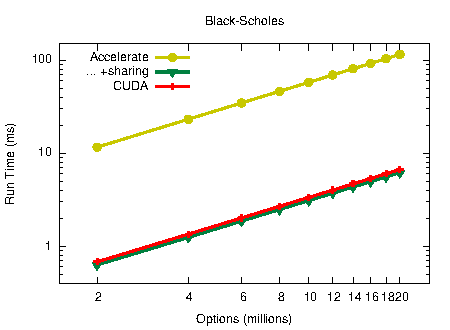
\includegraphics[width=0.8\textwidth]{images/results/black-scholes/black-scholes}
    \end{center}
    \caption[Black-Scholes kernel benchmarks]{Kernel runtimes for Black-Scholes
        options pricing, in Accelerate with and without optimisations, compared
        to a hand-written CUDA version. Note the log-log scale.}
    \label{fig:blackscholes}
\end{figure}

\subsection{Too little sharing}

The function @callput@ from Listing~\ref{lst:blackscholes} includes a
significant amount of sharing: the helper functions @cnd'@ and hence
@horner@ are used twice --- for @d1@ and @d2@ --- and its
argument @d@ is used multiple times in the body. Furthermore, the
conditional expression @d >* 0 ? (1 - c, c)@ results in a branch that,
without sharing, results in a growing number of predicated instructions that
leads to a large penalty on the SIMD architecture of the GPU\@.

Without sharing the generated code requires 5156 instructions to calculate 128
options (2 thread blocks of 64 threads each) and results in significant warp
divergence which serialises portions of the execution. With sharing recovery the
generated code requires 628 instructions (one thread block of 128 threads each)
and is actually slightly faster than the reference CUDA version because the
latter contains a common subexpression that was not spotted by the programmer,
and not eliminated by the CUDA compiler. The common subexpression performs a
single multiplication. The CUDA version executes 652 instructions (one thread
block of 128 threads each).


\section{Mandelbrot fractal}
\label{sec:mandelbrot}

The Mandelbrot set is generated by sampling values $c$ in the complex plane and
determining whether under iteration of the complex quadratic polynomial:
\[
z_{n+1} = z_{n}^{2} + c
\]
that the magnitude of $z$ (written $\left| z_{n} \right|$) remains bounded
however large $n$ gets. Images of the Mandelbrot set are created such that each
pixel corresponds to a point $c$ in the complex plane, and its colour depends on
the number of iterations $n$ before the relation diverges, where $z_{0} = c$.
The set of points forming the boundary of this relation forms the distinctive
and easily recognisable fractal shape shown in Figure~\ref{fig:mandelbrot}.

\begin{figure}
    \begin{center}
        
\includegraphics[width=0.8\textwidth]{images/results/mandelbrot/mandelbrot}
    \end{center}
    \caption[The Mandelbrot fractal]{Image of a Mandelbrot set with a
        continuously coloured environment. Each pixel corresponds to a point $c$
        in the complex plane, and its colour depends the number of iterations
        $n$ before the relation diverges. Centre coordinate
        $\left( -0.5+0i \right)$, horizontal width 3.2.}
    \label{fig:mandelbrot}
\end{figure}

\begin{table}
\centering
\small
\begin{tabu}{lrrrr}
\toprule

                        & \multicolumn{1}{c}{\textbf{Time}}
                        & \multicolumn{1}{c}{\textbf{Bandwidth}}
                        & \multicolumn{1}{c}{\textbf{Step}}
                        & \multicolumn{1}{c}{\textbf{Cumulative}} \\

\textbf{Benchmark}      & \multicolumn{1}{c}{\textbf{(ms)}}
                        & \multicolumn{1}{c}{\textbf{(GB/s)}}
                        & \multicolumn{1}{c}{\textbf{Speedup}}
                        & \multicolumn{1}{c}{\textbf{Speedup}} \\\midrule

Accelerate              & 430.77
                        & 0.018
                        &
                        & \\

Accelerate (+sharing)   & 426.18
                        & 0.018
                        & 1.01$\times$
                        & 1.01$\times$ \\

Accelerate (+fusion)    & 16.10
                        & 0.48
                        & 26.5$\times$
                        & 26.8$\times$ \\

Accelerate (+loop recovery)
                        & 20.17
                        & 0.38
                        & 0.80$\times$
                        & 21.4$\times$ \\

Accelerate (+iteration)
                        & 7.61
                        & 1.01
                        & 2.65$\times$
                        & 56.6$\times$ \\[0.5ex]

CUDA (limit)            & 13.97
                        & 0.55
                        &
                        & \\

CUDA (avg)              & 4.99
                        & 1.54
                        & 2.79$\times$
                        & 2.79$\times$ \\[0.5ex]

% C (avg)                 & 1389
%                         & 0.006
%                         &
%                         & \\[0.5ex]

Repa (-N8)              & 142.87
                        & 0.054
                        &
                        & \\

\bottomrule
\end{tabu}
\caption[Mandelbrot fractal kernel benchmarks]{Mandelbrot fractal benchmarks in
    Accelerate with and without optimisations, compared to a hand written CUDA
    version. The benchmark computes the Mandelbrot set shown in
    Figure~\ref{fig:mandelbrot}
    % , which has centre coordinates $-0.7 + 0i$ and width $3.067$
    at a resolution of $1600\times1200$. The CUDA (limit) benchmark computes
    every pixel to the maximum iteration count.}
\label{tab:mandelbrot}
\end{table}

Table~\ref{tab:mandelbrot} shows the results of the Mandelbrot program. As
expected, without fusion the performance of this benchmark is poor because
storing each step of the iteration saturates the memory bus, to the point that
reducing arithmetic intensity with sharing recovery provides no improvement.


\subsection{Fixed unrolling}

In order to meet the restrictions of what can be efficiently executed on
specialised hardware such as GPUs, Accelerate did not directly support any form
of iteration or recursion. To implement the recurrence relation we instead
define each step of computing $z_{n+1}$ given $z_n$ and $c$ as a collective
operation, and apply the operation a fixed number of times. The trick then is to
keep a pair @(z, i)@ for every point on the complex plane, where @i@ is the
iteration at which the point @z@ diverged. The code implementing this is shown
in Listing~\ref{lst:mandelbrot}.

\begin{lstlisting}[style=haskell_float
    ,label=lst:mandelbrot
    ,caption={Mandelbrot set generator, using fixed unrolling}]
mandelbrot
    :: forall a. (Elt a, IsFloating a)
    => Int
    -> Int
    -> Int
    -> Acc (Scalar (View a))
    -> Acc (Array DIM2 Int32)
mandelbrot screenX screenY depth view
  = P.snd . A.unzip
  $ P.foldr ($) zs0                                                                    -- (1)
  $ P.take depth (repeat step)
  where
    -- The view plane
    (xmin,ymin,xmax,ymax)     = unlift (the view)
    sizex                     = xmax - xmin
    sizey                     = ymax - ymin
    viewx                     = constant (P.fromIntegral screenX)
    viewy                     = constant (P.fromIntegral screenY)

    step :: Acc (Array DIM2 (Complex a, Int32))
         -> Acc (Array DIM2 (Complex a, Int32))
    step = A.zipWith iter cs

    iter :: Exp (Complex a) -> Exp (Complex a, Int32) -> Exp (Complex a, Int32)        -- (2)
    iter c zi = next (A.fst zi) (A.snd zi)
     where
      next :: Exp (Complex a) -> Exp Int32 -> Exp (Complex a, Int32)
      next z i =
        let z' = c + z*z
        in (dot z' >* 4) ? ( zi , lift (z', i+1) )                                     -- (3)

    dot :: Exp (Complex a) -> Exp a
    dot c = let r :+ i = unlift c
            in  r*r + i*i

    -- initial conditions for a given pixel in the window, translated to the
    -- corresponding point in the complex plane
    cs  = A.generate (constant $ Z :. screenY :. screenX) initial
    zs0 = A.map (\c -> lift (c, constant 0)) cs

    initial :: Exp DIM2 -> Exp (Complex a)
    initial ix = lift ( (xmin + (x * sizex) / viewx) :+ (ymin + (y * sizey) / viewy) )
      where
        pr = unindex2 ix
        x  = A.fromIntegral (A.snd pr :: Exp Int)
        y  = A.fromIntegral (A.fst pr :: Exp Int)
\end{lstlisting}

\begin{enumerate}
\item The function @step@ advances the entire complex plane by one iteration of
    the recurrence relation. This function is repeated @depth@ number of times,
    and the sequence combined by folding together with function application
    @($)@. This effectively unrolls the loop to @depth@ iterations.

\item The function @iter@ computes the next value in the sequence for a single
    point on the complex plane. If the point has diverged, we return the
    iteration count at which divergence occurred, otherwise the new value @z'@
    is returned and the iteration count @i@ is increased.

\item The conditional test is performed by the @(?)@ operator. Recall that GPUs are
    designed to do the same thing to lots of different data at the same time,
    whereas we want to do something different depending on whether or not a
    particular point has diverged. While we can not avoid having some kind of
    conditional in the code, we ensure there is only a bounded amount of
    divergence by having just one conditional per iteration, and a fixed number
    of iterations.

\end{enumerate}

Array fusion applied to the program in Listing~\ref{lst:mandelbrot} results in
the @depth@ copies of the function @step@ being combined into a single kernel.
As seen in Table~\ref{tab:mandelbrot}, while fusion improves the performance of
this program, it is still slower than the hand written version.

This slowdown is because the fused code generates a completely unrolled loop,
with @depth@ copies of the function body. Unrolling loops not only increases
instruction counts, but can often increase register lifetimes because of the
scheduling of loads and stores. In particular, stores are pushed down and loads
moved up in the instruction stream, which results in temporary scalar lifetimes
being longer.%
\footnote{\label{ft:fixed_unrolling}Register usage depends on which architecture
the code is being compiled for. For the compute 1.3 series processor, each
thread required 29 registers, whereas on a newer 3.0 processor the same code
required 59 registers per thread. I conjecture that this is because older
devices use a different underlying compiler architecture (Open64 vs.\ LLVM).}
% The unrolled code requires 63 registers, resulting in a multiprocessor occupancy
% of 50\% on a compute 3.0 device.
Since the Mandelbrot program is limited by computation, reducing the number of
resident threads has a corresponding reduction on maximum performance.

% \begin{lstlisting}[style=cuda
%     ,firstnumber=24]
% const float v13 = v10 * v10 - v11 * v11;                // single application of \texttt{step}
% const float v14 = v10 * v11 + v11 * v10;
% const float v15 = v8 + v13;
% const float v16 = v9 + v14;
% const Word8 v17 = v15 * v15 + v16 * v16 > 4.0f;
% const float v18 = v17 ? v10 : v15;
% const float v19 = v17 ? v11 : v16;
% const Int64 v20 = v17 ? v12 : (Int64) 1;
%   // repeats 255 times\ldots
% \end{lstlisting}


\subsection{Loop recovery}
\label{sec:loop_recovery}

Loop unrolling or loop unwinding is a loop transformation technique that
attempts to optimise a program's execution speed by reducing or eliminating
instructions that control the loop, such as branching and the end-of-loop test.
Loop unrolling does not always improve performance, however, because it may lead
to, for example, increased register usage.

Applying the fusion transformation to the Mandelbrot program shown in
Listing~\ref{lst:mandelbrot} resulted in a single kernel with @depth@ copies of
the function @iter@. In essence, the loop computing the Mandelbrot recurrence
relation has been completely unrolled. Unfortunately, the fused program does not
match the performance of the hand written version, because (a)
The program has a increased register usage; and (b) the conditional test is
still performed at the end of each copy of the loop body, so there is no
reduction in the overall number of instructions and branches executed.

We attempted to reduce these overheads by re-introducing explicit scalar loops
into the generated code. Recovering scalar loops then enables a backend to
generate explicit @for@ loops in the target language, and the compiler then
makes the decision of whether or not to unroll the loop. The following pair of
rewrite rules are used.
%
\begin{lstlisting}[style=Haskell,numbers=none,mathescape]
%\bf$\langle$ loop introduction $\rangle$%
    let x =
        let y = e1
        in e2
    in e3
    $\mapsto$
    iterate[2] (\y -> e2) e1            %\rm if \texttt{e2} $\equiv$ \texttt{e3}%

%\bf$\langle$ loop joining $\rangle$%
    let x = iterate[n] (\y -> e2) e1
    in e3
    $\mapsto$
    iterate[n+1] (\y -> e2) e1          %\rm if \texttt{e2} $\equiv$ \texttt{e3}%
\end{lstlisting}

As seen in Table~\ref{tab:mandelbrot}, loop recovery did not result in improved
performance in this case, because of the introduction of extra instructions to
track the iteration count of the loop.%
\footnote{As noted in footnote~\ref{ft:fixed_unrolling}, the CUDA compiler
produces code with different register usage patterns depending on which
architecture is being targeted. For newer devices that exhibited higher register
usage when compiling completely unrolled code, loop recovery provided good
increases in performance, by reducing register usage and thereby increasing
multiprocessor occupancy.}
Both the unrolled and loop recovery methods are slower than the hand written
program, because every thread always executes until the iteration limit.

% loop recovery shows a good increase in
% performance compared to the fused and unrolled result, but is slower than the
% hand written CUDA program because every thread always executes until the
% iteration limit, even if it diverges immediately, and must maintain this extra
% information of whether or not the thread has diverged yet.


\subsection{Explicit iteration}

Although not yet appearing in any published materials, we have added
explicit value recursion constructs to the source and target languages. Robert
Clifton-Everest implemented the necessary changes to the sharing recovery
algorithm, while I implemented the backend changes for code generation and
execution. The new function @while@ applies the given function, starting with
the initial value, as long as the test function continues to evaluate to @True@.
%
\begin{lstlisting}[style=haskell]
while :: Elt e
      => (Exp e -> Exp Bool)            -- conditional test
      -> (Exp e -> Exp e)               -- function to iterate
      -> Exp e                          -- initial value
      -> Exp e
\end{lstlisting}
%
The Mandelbrot program using explicit iteration is shown in
Listing~\ref{lst:mandelbrot_loop}, where the common parts to the @where@ clause
in Listing~\ref{lst:mandelbrot} have been elided. Note that in contrast to the
implementation based on fixed unrolling, the function will stop executing as
soon as the relation diverges, rather than always continuing to the iteration
limit even if the point has already diverged.

\begin{lstlisting}[style=haskell_float
    ,label=lst:mandelbrot_loop
    ,caption={Mandelbrot set generator, using explict iteration}]
mandelbrot
    :: forall a. (Elt a, IsFloating a)
    => Int
    -> Int
    -> Int
    -> Acc (Scalar (View a))
    -> Acc (Array DIM2 Int32)
mandelbrot screenX screenY depth view =
  generate (constant (Z :. screenY :. screenX))
           (\ix -> let c = initial ix
                   in  A.snd $ A.while (\zi -> A.snd zi <* lIMIT &&* dot (A.fst zi) <* 4)
                                       (\zi -> lift1 (next c) zi)
                                       (lift (c, constant 0)))
  where
    lIMIT = P.fromIntegral depth

    next :: Exp (Complex a) -> (Exp (Complex a), Exp Int32) -> (Exp (Complex a), Exp Int32)
    next c (z, i) = (c + (z * z), i+1)
\end{lstlisting}

With respect to implementation on SIMD architectures such as CUDA, while both
the fixed unrolling and explicit iteration methods have a conditional test that
introduces thread divergence, it is important to note that the behaviour of the
divergence is different for each method. In the fixed unrolling case, both
branches of the conditional must be executed to keep track of whether the
element has already diverged. This results in threads following separate
execution paths, where threads that follow the @True@ branch execute while all
other threads sit idle, then execution switches to the @False@ branch and the
first set of threads sit idle. In contrast, in the explicit iteration case,
threads exit the loop as soon as their point on the complex plane diverges, and
then simply wait for all other threads in their SIMD group to complete their
calculation and catch up.

While the introduction of explicit value recursion required changes to the
source language program, as seen in Table~\ref{tab:mandelbrot}, performance
improves significantly. Additionally, if all threads in the SIMD group diverge
quickly, this can save a significant amount of redundant computation.
Table~\ref{tab:mandelbrot} also shows the difference in execution time between
computing the entire fractal shown in Figure~\ref{fig:mandelbrot}, where all
points diverge at different depths in the sequence (avg), compared to a region
where all threads continue to the iteration limit (limit).


\subsection{Unbalanced workload}

In order to manage the unbalanced workload inherent in the Mandelbrot
computation, the hand-written CUDA version includes a custom, software-based
thread-block scheduler, an idea which has gained recent popularity under the
name of persistent threads~\cite{Gupta:2014ik}. In this vein, future work could
investigate adding a software-based load balancing scheduler to the generated
kernels, perhaps based on ideas of work
stealing~\cite{Randall:1998,Tzannes:2010il}, instead of statically partitioning
the work space. An orthogonal line of work is that of generating kernel code
that avoids thread divergence, which is an active area of
research~\cite{Zhang:2010jc}.

% The final problem with the Mandelbrot program is due to the initial formulation
% of the program using a fixed unrolling, as we must handle application of the
% function to elements which have already diverged. As explained, this is to
% ensure that all threads [in a warp] continue doing the same thing, which avoids
% excessive SIMD divergence, but means that the computation always proceeds to the
% iteration limit.
%
% For the Mandelbrot program threads only diverge in the sense that they are
% either still computing the recurrence relation, or the point is not in the set
% and the computation has completed; threads do not diverge to follow separate
% execution paths. The latter type of SIMD divergence is what we really need to
% avoid, because this results in predicated execution: threads taking the
% @true@ path of a branch execute while all other threads sit idle, then
% execution switches to the @false@ branch while the first set of threads
% idle.
%
% The CUDA version is faster because threads exit the loop as soon as their point
% in the complex plane diverges. Although once a thread completes it sits idle
% until all threads in the group complete their calculation, if all the points
% within a group of threads diverge quickly this can save a significant amount of
% work. Table~\ref{tab:mandelbrot} shows the difference in execution time when
% displaying the entire fractal (avg), where points diverge at varying iteration
% depths in the sequence, compared to a region where all thread continue to the
% iteration limit (limit). In order to manage this unbalanced workload, the CUDA
% version additionally includes a custom thread block scheduler.
%
% This test demonstrates that while loop recovery offered a significant
% performance benefit for free, it would be beneficial to expose looping
% constructs in the source language as well, rather than relying on potentially
% fragile post-hoc transformations. Avoiding thread divergence in CUDA programs is
% an active area of research~\cite{Zhang:2010jc}.

\subsection{Passing inputs as arrays}

Note that in the definition of @mandelbrot@, the current view bounds are passed
as a scalar array. Why don't we pass these values as plain @Float@s? When the
program runs, Accelerate converts the program into a series of CUDA kernels,
each of which must be compiled and loaded onto the
GPU~(\S\ref{sec:code_generation}). Since compilation can take a while,
Accelerate remembers the kernels it has seen before and reuses
them~(\S\ref{sec:dynamic_compilation}). Our goal with @mandelbrot@ is to make a
kernel that will be reused, otherwise the overhead of compiling a new kernel
each time the view is changed will ruin performance.

By defining the @view@ as a scalar array, we ensure that it is defined
\emph{outside} the call to @generate@. If we don't do this, a different value
for the view parameter will be embedded directly into each call to the
@generate@ function, which will defeat Accelerate's caching of CUDA kernels.

Any scalar values that we wish to be treated as function parameters must be
lifted to array variables. This is because the internal representation of array
terms is closed with respect to scalar variables, in order to statically exclude
nested parallelism. Adding support for nested data parallelism to Accelerate is
an active area of research. With it, it may be possible to avoid lifting free
scalar variables to free array variables in order to correctly cache kernels.


\section{N-body gravitational simulation}
\label{sec:nbody}

\begin{figure}
    \begin{center}
        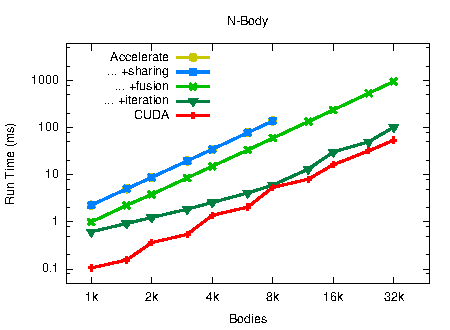
\includegraphics[width=0.8\textwidth]{images/results/nbody/nbody}
    \end{center}
    \caption[N-body gravitational simulation kernel benchmarks]{Kernel runtimes
        for the $n$-body gravitational simulation, in Accelerate with and
        without optimisations, compared to a hand-written CUDA implementation.
        Note the log-log scale.}
    \label{fig:nbody}
\end{figure}

The $n$-body example simulates the Newtonian gravitational forces on a set of
massive bodies in 3D space, using the na\"ive $\mathcal{O}\left( n^{2} \right)$
algorithm. In a data-parallel setting, the natural way to express this algorithm
is first to compute the forces between every pair of bodies, before adding the
forces applied to each body using a segmented sum. Without fusion this approach
also requires $\mathcal{O}\left( n^{2} \right)$ space for the intermediate array
of forces, which exhausts the memory of our device (4GB!) when using more than
about five thousand bodies. With fusion, the reduction operation consumes each
force value on-the-fly, so that the program only needs $\mathcal{O}\left( n
\right)$ space to store the final force values. The core of the $n$-body
simulation is shown in Listing~\ref{lst:nbody}, where @accel@ calculates
the acceleration between two particles, and @(.+.)@ component-wise sums the
acceleration of a particle along each $x$, $y$ and $z$ axis.

\begin{lstlisting}[style=haskell_float
    ,label=lst:nbody
    ,caption={$N$-body gravitational simulation, using parallel reduction}]
calcAccels :: Exp Float -> Acc (Vector Body) -> Acc (Vector Accel)
calcAccels epsilon bodies
  = let n       = A.size bodies
        cols    = A.replicate (lift $ Z :. n :. All) bodies
        rows    = A.replicate (lift $ Z :. All :. n) bodies
    in
    A.fold (.+.) (vec 0) $ A.zipWith (accel epsilon) rows cols
\end{lstlisting}


\subsection{Sequential iteration}

Even with fusion, the reference CUDA version is over $10\times$ faster. Although
the fused program requires only $\mathcal{O}\left( n \right)$ space, it still
requires all $\mathcal{O}\left( n^2 \right)$ memory accesses, and $n^{2}$
threads to cooperatively compute the interactions.

With the addition of sequential iteration, we can emit an alternative
implementation. Rather than computing all interactions between each pair of
bodies and reducing this array in parallel, we express the program as a parallel
map of sequential reductions, as shown in Listing~\ref{lst:nbody_seq}. Although
the program still performs all $n^{2}$ memory accesses, since all threads access
the @bodies@ array in sequence, these values can be cached efficiently by the
GPU, and the actual bandwidth requirements to main memory are reduced.

\begin{lstlisting}[style=haskell_float
    ,label=lst:nbody_seq
    ,caption={$N$-body gravitational simulation, using sequential reduction}]
calcAccels :: Exp R -> Acc (Vector PointMass) -> Acc (Vector Accel)
calcAccels epsilon bodies
  = let move body = A.sfoldl (\acc next -> acc .+. accel epsilon body next)
                             (vec 0)
                             (constant Z)
                             bodies
    in
    A.map move bodies
\end{lstlisting}


\subsection{Use of shared memory}

In CUDA, the memory hierarchy of the device is made explicit to the programmer,
including a small on-chip shared memory\cuda[shared memory]{} region threads can
use to share data. The shared memory region is essentially a software managed
cache~\cite{NVIDIA:2012wf}.

The program shown in Listing~\ref{lst:nbody} uses the shared memory region to
share computations while computing the parallel reduction.\footnote{As part of
the second phase of the \footcode{fold} skeleton, where threads in a block
cooperatively reduce elements to a single value. See
\S\ref{sec:parallel_reduction} for details.}
The second implementation shown in Listing~\ref{lst:nbody_seq} does not use
shared memory at all, but rather relies on hardware caching. Similar to our
latter implementation, the CUDA program is also implemented as a parallel map of
sequential reductions, but explicitly uses the shared memory region to share the
particle mass and position data between threads, rather than rely on hardware
caching. Since the shared memory region is very low latency, the CUDA program
remains faster. Automatic use of shared memory is a separate consideration to
the optimisations discussed in this work, and remains an open research
problem~\cite{Ma:2010ft}.

% This reduces the bandwidth requirement of the program by a factor of the number
% of threads in a block (256) but requires each thread to sum its particle
% interactions sequentially in $\mathcal{O}\left( n \right)$ time. The Accelerate
% version uses shared memory to perform a tree-reduction in $\mathcal{O}\left(
% \log n \right)$ time (\S\ref{sec:parallel_reduction}) but requires all $n^{2}$
% memory transfers. For this bandwidth bound application, making the trade-off of
% parallelism for bandwidth clearly wins. Automatic use of shared memory is a
% separate consideration to the optimisations discussed in this work, and remains
% an open research problem~\cite{Ma:2010ft}.


\section{Sparse-matrix vector multiplication}
\label{sec:smvm}

\newcommand\spyplot[1]{\parbox[c][1.1cm][c]{1.1cm}{\includegraphics[width=1cm]{images/results/smvm/#1}}}

\begin{table}
\centering
\small
\begin{tabu}{X[-1cm]X[2lm]cX[-1cb]rrrr} \toprule

\textbf{spyplot}
& \textbf{Description}
& \textbf{Dimensions}
& \textbf{Nonzeros (nnz/row)}
& \multicolumn{1}{c}{\rotatebox{90}{\textbf{Accelerate}}}
& \multicolumn{1}{c}{\begin{sideways}%
    \parbox{\widthof{\bf Accelerate}}%
    {\centering\textbf{Accelerate no fusion}}%
    \end{sideways}}
& \multicolumn{1}{c}{\rotatebox{90}{\textbf{CUSP}}}
& \multicolumn{1}{c}{\rotatebox{90}{\textbf{CUSPARSE}}}
\\ \midrule

\spyplot{dense2} % Dense
& Dense matrix in sparse format
& 2K $\times$ 2K
& 4.0M (2K)
& 15.55 & 5.82 & 11.8 & 0.06
% & 14.48 & 14.62 & 3.41
\\

\spyplot{pdb1HYS} % Protein
& Protein data bank 1HYS
& 36K $\times$ 36K
& 2.19M (60)
& 7.59 & 3.89 & 4.16 & 0.03
% & 13.55 & 13.65 & 0.26
\\

\spyplot{consph} % FEM / Spheres
& FEM/Concentric spheres
& 83K $\times$ 83K
& 3.05M (37)
& 4.93 & 1.92 & 3.67 & 0.04
% & 12.63 & 9.03 & 4.70
\\

\spyplot{cant} % FEM / Cantilever
& FEM/Cantilever
& 62K $\times$ 62K
& 2.03M (33)
& 4.46 & 2.37 & 3.37 & 0.94
% & 11.98 & 7.96 & 4.41
\\

\spyplot{pwtk} % Wind Tunnel
& Pressurised wind tunnel
& 128K $\times$ 128K
& 5.93M (27)
& 3.99 & 1.40 & 3.80 & 0.02
% & 11.98 & 7.33 & 4.62
\\

\spyplot{rma10} % FEM/Harbour
& FEM/Charleston harbour
& 47K $\times$ 47K
& 2.37M (50)
& 6.70 & 3.60 & 7.03 & 0.02
% & 9.42 & 6.14 & 0.13
\\

\spyplot{qcd5_4} % QCD
& Quark propagators (QCD/LGT)
& 49K $\times$ 49K
& 1.92M (39)
& 5.07 & 3.03 & 5.45 & 0.02
% & 7.79 & 4.66 & 0.13
\\

\spyplot{shipsec1} % FEM/Ship
& FEM/Ship section detail
& 141K $\times$ 141K
& 3.98M (28)
& 4.03 & 1.82 & 3.61 & 0.08
% & 12.28 & 6.60 & 4.47
\\

\spyplot{mac_econ_fwd500} % Economics
& Macroeconomics model
& 207K $\times$ 207K
& 1.27M (6)
& 0.97 & 0.61 & 2.91 & 0.04
% & 4.59 & 0.90 & 1.06
\\

\spyplot{mc2dephi} % Epidemiology
& 2D Markov epidemiology model
& 526K $\times$ 526K
& 2.10M (4)
& 0.64 & 0.29 & 5.62 & 0.74
% & 6.42 & 0.59 & 0.91
\\

\spyplot{cop20k_A} % FEM/Accelerator
& FEM/Accelerator cavity design
& 121K $\times$ 121K
& 1.36M (11)
& 1.72 & 1.20 & 2.12 & 0.04
% & 5.41 & 3.08 & 2.92
\\

\spyplot{scircuit} % Circuit
& Circuit simulation
& 171K $\times$ 171K
& 959k (6)
& 0.87 & 0.60 & 3.24 & 0.01
% & 3.56 & 0.82 & 1.08
\\

\spyplot{webbase-1M} % Webbase
& Web connectivity matrix
& 1M $\times$ 1M
& 3.11M (3)
& 0.50 & 0.20 & 2.01 & 0.01
% & 2.11 & 0.47 & 0.74
\\

\spyplot{rail4284} % LP
& Railways set cover constraint matrix
& 4K $\times$ 1.1M
& 11.3M (2633)
& 5.08 & 3.64 & 5.16 & 0.07
% & 5.22 & 5.04 & 2.41
\\

\bottomrule
\end{tabu}
\caption[Sparse-matrix vector multiplication benchmarks]{Overview of sparse
matrices tested and results of the benchmark. Measurements are in GFLOPS/s
(higher is better).}
\label{tab:smvm_summary}
\end{table}


This benchmark considers the multiplication of sparse matrices in compressed row
format (CSR)~\cite{Chatterjee:1990vj} with a dense vector. This matrix format
consists of an array of the non-zero elements paired with their column index,
together with a segment descriptor recording the number of non-zeros in each
row. The corresponding Accelerate code is shown in Listing~\ref{lst:smvm}.
Table~\ref{tab:smvm_summary} compares Accelerate to the CUSP
library~\cite{Bell:2008wc,Bell:2009bl}, a special purpose library for sparse
matrix operations (version 0.4), and the CUSPARSE library which is part of the
NVIDIA CUDA distribution. Using a 14 matrix corpus derived from a variety of
application domains~\cite{Williams:2009cy}, we compare against using compressed
row format matrices. The measured times include only the core sparse matrix
multiply operation.

\begin{lstlisting}[style=haskell
    ,float
    ,label=lst:smvm
    ,caption={Sparse-matrix vector multiplication}]
type SparseVector e = Vector (Int, e)                   -- column index and value
type SparseMatrix e = (Segments Int, SparseVector e)    -- length of each row

smvm :: (Elt a, IsNum a) => Acc (SparseMatrix a) -> Acc (Vector a) -> Acc (Vector a)
smvm smat vec
  = let (segd, svec)    = unlift smat
        (inds, vals)    = A.unzip svec
        vecVals         = gather inds vec
        products        = A.zipWith (*) vecVals vals
    in
    foldSeg (+) 0 products segd
\end{lstlisting}

Compared to our previous work~\cite{Chakravarty:2011fr} the fusion
transformation compresses the program into a single segmented reduction. As
predicted, the corresponding reduction in memory bandwidth means that Accelerate
is on par with the CUSP library for several of the test matrices. In a balanced
machine SMVM should be limited by memory throughput, so a dense matrix in
sparse format should provide an upper bound on performance because loops are
long running and accesses to the source vector are contiguous and have high
re-use. We see that Accelerate with array fusion achieves this expected
performance limit. For some benchmarks Accelerate is significantly faster than
CUSP, while in others it lags behind. It is unknown why the NVIDIA
CUSPARSE library is significantly slower on all test matrices.
%, but is also slightly faster than the CUSP implementation.

\subsection{Segment startup}

To maximise global memory throughput, the skeleton code ensures that the vector
read of each matrix row is coalesced and aligned to the warp boundary. Combined
with the behaviour that reduction operations in Accelerate do not require a
neutral starting element, this means that there is significant overhead in
initialising the local sum for each thread at the beginning of the reduction.
See Section~\ref{sec:dotp} for further discussion.

% Since Accelerate does not require the starting element of the reduction to be a
% neutral element, threads must also ensure they initialise their local sum from
% the input array (\ref{sec:non-neutral_starting_elements}).
% Listing~\ref{lst:smvm_cuda} shows the generated CUDA code for the first
% sequential phase of the cascaded tree-reduction algorithm (see
% \S\ref{sec:algorithm_cascading}). Figure~tk illustrates the different cases that
% must be considered.
%
% \begin{lstlisting}[style=cuda_float
%     ,firstnumber=44
%     ,label=lst:smvm_cuda
%     ,caption={Generated CUDA code for sparse-matrix vector multiplication}]
% if (num_elements > warpSize) {
%     ix = start - (start & warpSize - 1) + thread_lane;                  (@* \label{lst:smvm_cuda_boundary} *@)
%     if (ix >= start) {                                                  (@* \label{lst:smvm_cuda_warp_start} *@)
%         const Int64 v3 = ix;
%         const int v4 = toIndex(shIn2, shape(v3));
%         const int v5 = toIndex(shIn1, shape((Int64) arrIn2_a1[v4]));
%         const int v6 = toIndex(shIn2, shape(v3));
%
%         y0 = arrIn1_a0[v5] * arrIn2_a0[v6];
%     }
%     if (ix + warpSize < end) {                                          (@* \label{lst:smvm_cuda_warp_next} *@)
%         const Int64 v3 = ix + warpSize;
%         const int v4 = toIndex(shIn2, shape(v3));
%         const int v5 = toIndex(shIn1, shape((Int64) arrIn2_a1[v4]));
%         const int v6 = toIndex(shIn2, shape(v3));
%
%         x0 = arrIn1_a0[v5] * arrIn2_a0[v6];
%         if (ix >= start) {                                              (@* \label{lst:smvm_cuda_branch} *@)
%             y0 = x0 + y0;
%         } else {
%             y0 = x0;
%         }
%     }
%     for (ix += 2 * warpSize; ix < end; ix += warpSize) {                (@* \label{lst:smvm_cuda_loop} *@)
%         const Int64 v3 = ix;
%         const int v4 = toIndex(shIn2, shape(v3));
%         const int v5 = toIndex(shIn1, shape((Int64) arrIn2_a1[v4]));
%         const int v6 = toIndex(shIn2, shape(v3));
%
%         x0 = arrIn1_a0[v5] * arrIn2_a0[v6];
%         y0 = x0 + y0;
%     }
% } else if (start + thread_lane < end) {                                 (@* \label{lst:smvm_cuda_unaligned} *@)
%     const Int64 v3 = start + thread_lane;
%     const int v4 = toIndex(shIn2, shape(v3));
%     const int v5 = toIndex(shIn1, shape((Int64) arrIn2_a1[v4]));
%     const int v6 = toIndex(shIn2, shape(v3));
%
%     y0 = arrIn1_a0[v5] * arrIn2_a0[v6];
% }
% \end{lstlisting}
%
% To initialise the warp-aligned read the location of the warp boundary before the
% start of the source vector is calculated (line~\ref{lst:smvm_cuda_boundary}),
% offset by this thread's warp lane index. If the thread lies within the source
% vector its starting value can be initialised
% (line~\ref{lst:smvm_cuda_warp_start}). Reading elements from the second warp
% (line~\ref{lst:smvm_cuda_warp_next}) is aligned and coalesced to the warp
% boundary so completes in a single global memory transfer, but requires a
% divergent branch (line~\ref{lst:smvm_cuda_branch}) depending on whether this is
% the first value read or not. Once all threads have initialised their local sum,
% the serial reduction phase completes (line~\ref{lst:smvm_cuda_loop}), which is
% the same as we saw in the dot product example (Listing~\ref{lst:dotp_cuda}). If
% there is less than a warp's worth of data to be reduced, the elements are simply
% read unaligned (line~\ref{lst:smvm_cuda_unaligned}). If we do not do this, the
% first threads of the warp may not have been initialised, which is a requirement
% for the second cooperative tree-reduction phase of the algorithm, as it combines
% values for indices $\left[0,n\right)$ into index zero.

For matrices such as Dense, the increase is memory bandwidth gained from
aligning global memory reads in this way offsets the additional startup cost of
doing so, and as a result Accelerate exhibits higher performance than its
competitors.
%
However, matrices such as the FEM/Spheres, which contain only a fewer non-zero
elements per row ($\lesssim 2 \times \text{warp size} = 64$) exhibit a drop in
performance, because this extra startup cost can not be amortised over the row
length.
%
Matrices such as Epidemiology, with large vectors and few non-zero elements per
row, exhibit low flop:byte ratio and are poorly suited to the CSR format, with
all implementations performing well below peak. This highlights the nature of
sparse computations and the reason the CUSP library supports several algorithms
and matrix formats.

As was found with the dot product benchmark (\S\ref{sec:dotp}), implementing
specialised kernels that can avoid this additional startup cost when the
combining function and starting element form a monoid is expected to improve
performance, but is left to future work.

% This may be related to the way the skeleton code ensures that
% the vector read of each row is coalesced and aligned to the warp boundary to
% maximise global memory throughput, but is then not able to amortize this extra
% startup cost over the row length.
%
% Since Accelerate does not require the starting element of the reduction to be a
% neutral element (see \S\ref{sec:non-neutral_starting_elements})
%
% The regression relative to
% our previous result will be investigated. Nevertheless,

\section{Canny edge detection}
\label{sec:canny}

The edge detection example applies the Canny algorithm~\cite{Canny:1986et} to
rectangular images of various sizes. Figure~\ref{fig:canny} compares Accelerate
to parallel implementations on the CPU and GPU\@. The overall algorithm is shown
in Listing~\ref{lst:canny} and consists of seven distinct phases, the first six
of which, shown in Listing~\ref{lst:canny-kernels}, are naturally data parallel
and are performed on the GPU\@. The last phase uses the recursive @wildfire@
algorithm to ``connect'' the pixels that make up the output lines. In our
implementation this phase is performed on the CPU, which requires the image data
to be transferred from the GPU back to the CPU for processing, and accounts for
the non-linear slowdown visible with smaller image sizes. In contrast,
OpenCV\footnote{Release version 2.4.9} is able to perform the final step on the
GPU\@. The benchmark ``Accelerate (whole program)'' includes the time to
transfer the image data back to the host for the final processing step. Also
shown are the run times for just the first six data parallel phases, which
exhibit linear speedup and do not include data transfer to the host.

\begin{figure}
    \begin{center}
        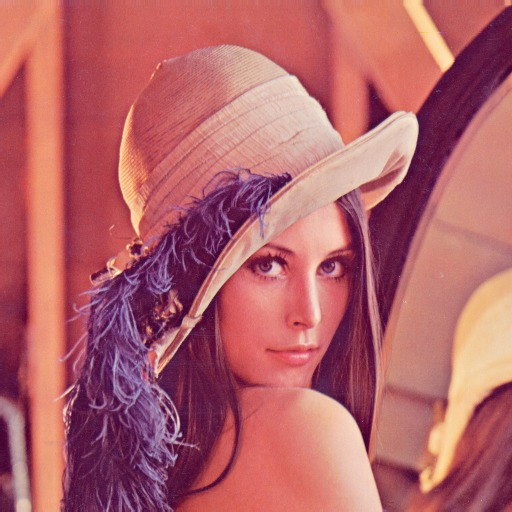
\includegraphics[width=0.45\textwidth]{images/results/canny/lena}
        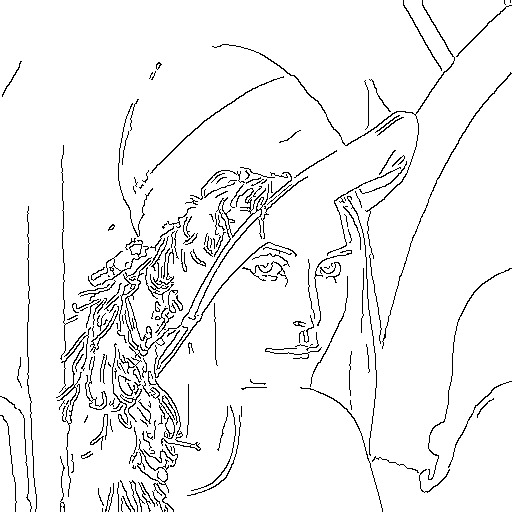
\includegraphics[width=0.45\textwidth]{images/results/canny/lena-edges}
    \end{center}
    \caption[Example of the Canny edge detection algorithm]{An example of the
        Canny algorithm applied to the Lena standard test image (left) which
        identifies edge pixels in the image (right).}
    \label{fig:lena}
\end{figure}

Neglecting the final phase, note that the data parallel phase is still slightly
slower than in OpenCV. As discussed in Section~\ref{sec:parallel_stencil}, this
is because the stencil kernels in Accelerate currently make a test for every
array access to see if the element is in bounds, or if it lies outside the array
and needs to be handled specially, even though the vast majority of points in
the array are far from the boundary.

\begin{figure}
    \begin{center}
        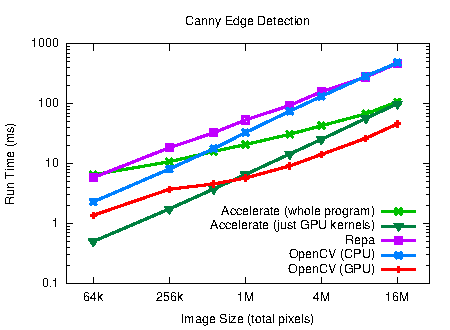
\includegraphics[width=0.8\textwidth]{images/results/canny/canny}
    \end{center}
    \caption[Canny edge detection benchmarks]{Runtimes for the Canny edge
        detection algorithm, comparing the Accelerate kernels and whole program
        to sequential and parallel implementations. Note the log-log scale.}
    \label{fig:canny}
\end{figure}

\begin{lstlisting}[style=haskell_float
    ,label=lst:canny
    ,caption={The Canny edge detection algorithm}]
canny :: Exp Float -> Exp Float -> Image -> IO Image
canny low high =
  let grey              = toGreyscale
      blurred           = gaussianY . gaussianX . grey
      magdir            = gradientMagDir low . blurred
      suppress          = nonMaximumSuppression low high . magdir
      stage1 x          = let s = suppress x in (s, selectStrong s)
      (image, strong)   = run $ A.lift (stage1 (use img))
  in
  wildfire (A.toRepa image) (A.toRepa strong)
\end{lstlisting}

\begin{lstlisting}[style=haskell_float
    ,label=lst:canny-kernels
    ,caption={The data-parallel kernels of the Canny edge detection algorithm}]
convolve5x1 :: (Elt a, IsNum a) => [Exp a] -> Stencil5x1 a -> Exp a
convolve5x1 kernel (_, (a,b,c,d,e), _)
  = P.sum $ P.zipWith (*) kernel [a,b,c,d,e]

gaussianX :: Acc (Image Float) -> Acc (Image Float)
gaussianX = stencil (convolve5x1 gaussian) Clamp
  where
    gaussian = P.map (/16) [ 1, 4, 6, 4, 1 ]

gradientX :: Acc (Image Float) -> Acc (Image Float)
gradientX = stencil grad Clamp
  where
    grad :: Stencil3x3 Float -> Exp Float
    grad ((u, _, x)
         ,(v, _, y)
         ,(w, _, z)) = x + (2*y) + z - u - (2*v) - w

gradientMagDir :: Exp Float -> Acc (Image Float) -> Acc (Array DIM2 (Float,Int))
gradientMagDir low = stencil magdir Clamp
  where
    magdir :: Stencil3x3 Float -> Exp (Float,Int)
    magdir ((v0, v1, v2)
           ,(v3,  _, v4)
           ,(v5, v6, v7)) =
      let
          dx          = v2 + (2*v4) + v7 - v0 - (2*v3) - v5     -- image gradients
          dy          = v0 + (2*v1) + v2 - v5 - (2*v6) - v7
          mag         = sqrt (dx * dx + dy * dy)                -- gradient magnitude
          theta       = atan2 dy dx                             -- angle of the gradient vector
          alpha       = (theta - (pi/8)) * (4/pi)               -- make segments easier to classify
          norm        = alpha + 8 * A.fromIntegral (boolToInt (alpha <=* 0))
          undef       = abs dx <=* low &&* abs dy <=* low
          dir         = boolToInt (A.not undef) *               -- quantise gradient to 8 directions
                            ((64 * (1 + A.floor norm `mod` 4)) `min` 255)
      in
      lift (mag, dir)

nonMaximumSuppression
  :: Exp Float -> Exp Float -> Acc (Image (Float,Int)) -> Acc (Image Float)
nonMaximumSuppression low high magdir =
  generate (shape magdir) $ \ix ->
    let (mag, dir)      = unlift (magdir ! ix)
        Z :. h :. w     = unlift (shape magdir)
        Z :. y :. x     = unlift ix

        -- Determine the points that lie normal to the image gradient
        offsetx         = dir >* orient' Vert  ? (-1, dir <* orient' Vert ? (1, 0))
        offsety         = dir <* orient' Horiz ? (-1, 0)
        (fwd, _)        = unlift $ magdir ! lift (clamp (Z :. y+offsety :. x+offsetx))
        (rev, _)        = unlift $ magdir ! lift (clamp (Z :. y-offsety :. x-offsetx))
        clamp (Z:.u:.v) = Z :. 0 `max` u `min` (h-1) :. 0 `max` v `min` (w-1)
        strong          = mag >=* high
        none            = dir ==* orient' Undef
                              ||* mag <* low ||* mag <* fwd ||* mag <* rev
    in
    A.fromIntegral (boolToInt (A.not none) * (1 + boolToInt strong)) * 0.5

selectStrong :: Acc (Image Float) -> Acc (Vector Int)
selectStrong img =
  let strong            = A.map (\x -> boolToInt (x ==* edge' Strong)) (flatten img)
      (targetIdx, len)  = A.scanl' (+) 0 strong
      indices           = A.enumFromN (index1 $ size img) 0
      zeros             = A.fill (index1 $ the len) 0
  in
  A.permute const zeros (\ix -> strong!ix ==* 0 ? (ignore, index1 $ targetIdx!ix)) indices
\end{lstlisting}


\subsection{Stencil merging}

Two of the data parallel stages of the Canny algorithm are the calculation of
the image intensity gradients by convolving the image with the $3\times3$
kernels shown below. This convolution, known as the Sobel operator, is a
discrete differentiation operator that computes an approximation of the
horizontal and vertical image gradients.
%
\begin{equation*}
    \text{Sobel}_x =
        \begin{bmatrix*}[r]
          -1 & 0 & 1 \\
          -2 & 0 & 2 \\
          -1 & 0 & 1
        \end{bmatrix*}
    \qquad
    \text{Sobel}_y =
        \begin{bmatrix*}[r]
           1 &  2 &  1 \\
           0 &  0 &  0 \\
          -1 & -2 & -1
        \end{bmatrix*}
\end{equation*}

There is a significant amount of sharing between these two kernels, in terms of
the coefficients required to compute the derivative at each point. Thus, it
is beneficial to merge these two stencils into a single kernel, rather
than computing them separately. This would reduce the number of accesses to the
source array from $6+6=12$ to only $8$. As with all shortcut fusion methods, the
system presented here does not combine multiple passes over the same array into
a single traversal that computes multiple results. We leave this, as well as
other significant stencil
optimisations~\cite{Henretty:2013wb,Kamil:2006un,Lesniak:2010}, to future work.

% We leave this to future work,
% for example, in the style of data flow fusion~\cite{Lippmeier:2013vz}.


\section{Fluid flow}
\label{sec:fluid}

The fluid flow example implements Jos Stam's stable fluid
algorithm~\cite{Stam:1999ey}, which is a fast approximate algorithm intended for
animation and games, rather than accurate engineering simulation. An example
sequence is shown in Figure~\ref{fig:fluid_steps}.

\begin{figure}
    \begin{center}
        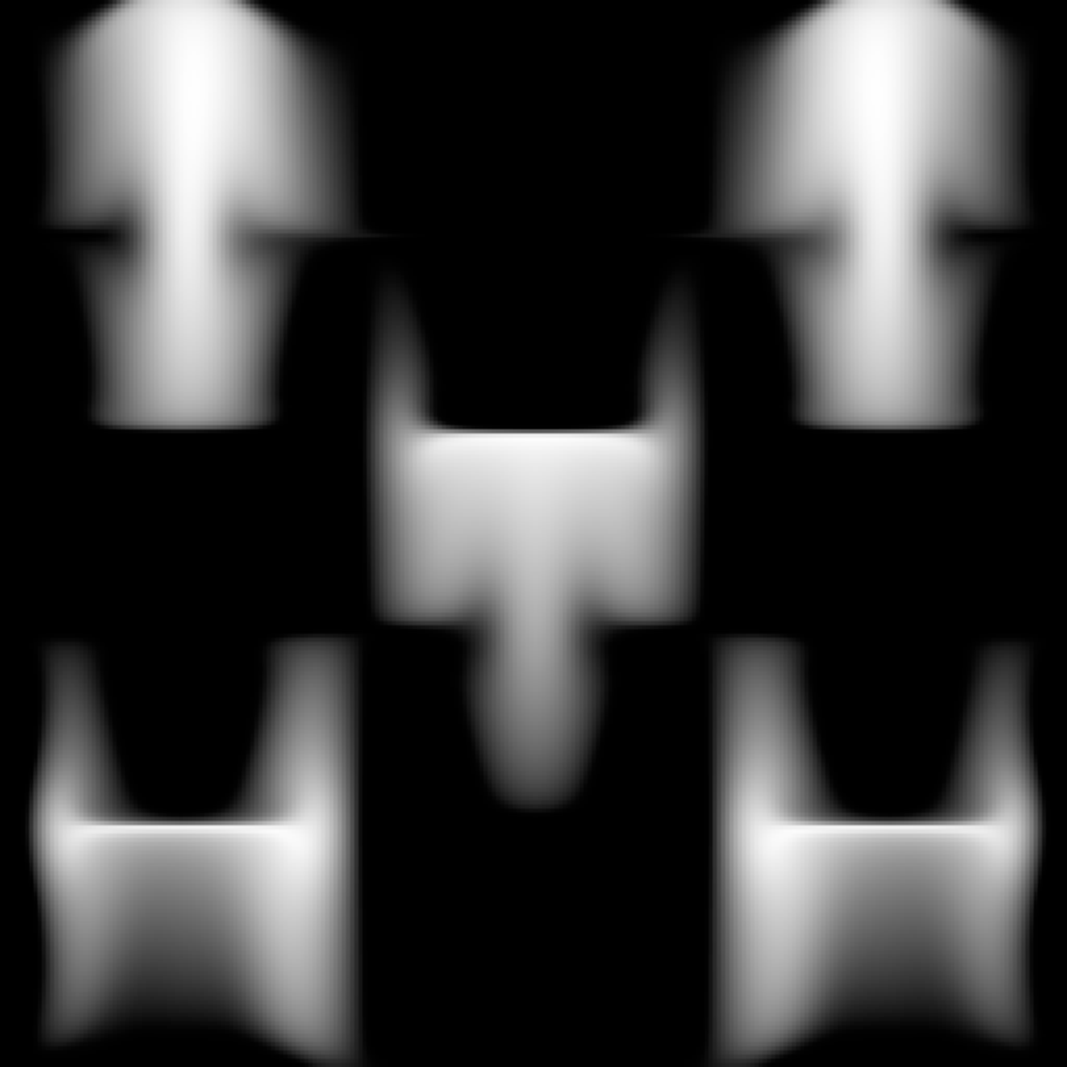
\includegraphics[width=0.3\textwidth]{images/results/fluid/fluid-10}
        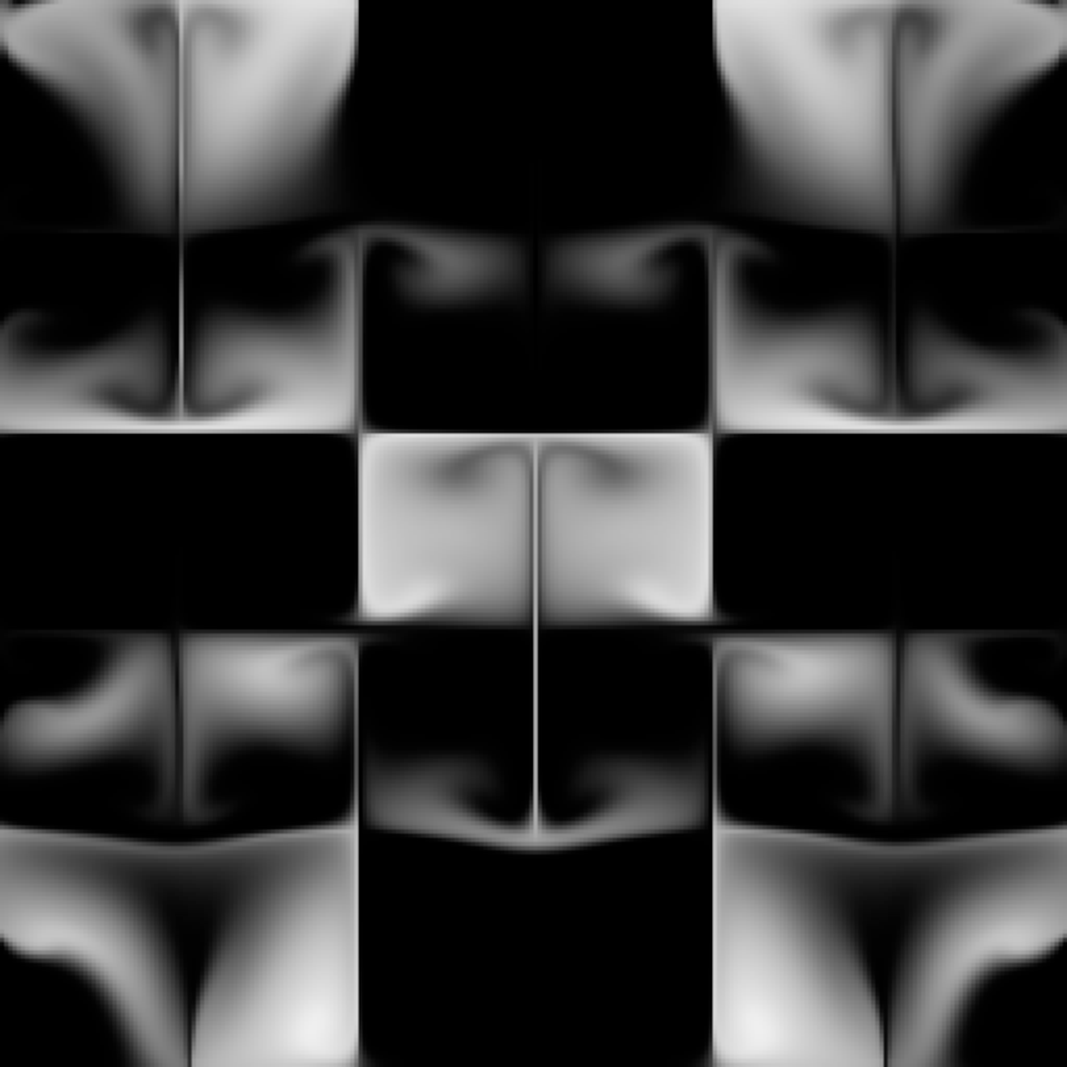
\includegraphics[width=0.3\textwidth]{images/results/fluid/fluid-50}
        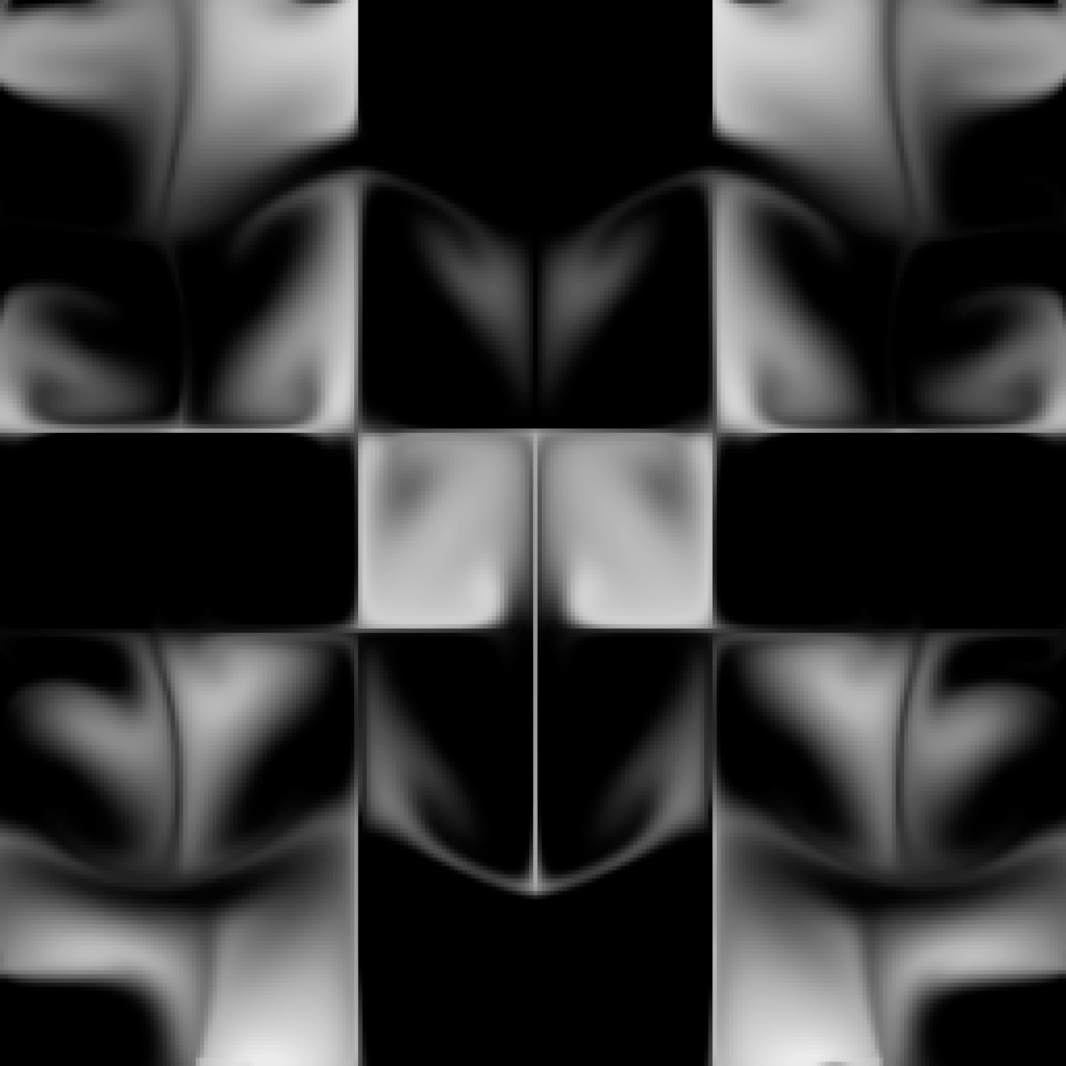
\includegraphics[width=0.3\textwidth]{images/results/fluid/fluid-75}
    \end{center}
    \caption[Example of the fluid flow simulation]{An example showing the
        progression of the fluid flow simulation for a set of initial conditions
        after 10 (left), 50 (centre) and 75 (right) steps.}
    \label{fig:fluid_steps}
\end{figure}

The core of the algorithm is a finite time step simulation on a grid,
implemented as a matrix relaxation involving the discrete Laplace operator
($\nabla^2$). This step, known as the linear solver, is used to diffuse the
density and velocity fields throughout the grid, as well as apply a projection
operator to the velocity field to ensure it conserves mass. The linear solver is
implemented in terms of a stencil convolution, repeatedly computing the
following for each grid element to allow the solution to converge:
\[
u_{i,j}^{''} = \left( u_{i,j} + a \cdot \left( u'_{i-1,j}+u'_{i+1,j}+u'_{i,j-1}+u'_{i,j+1} \right) \right) / c
\]
Here, $u$ is the grid in the previous time step, $u'$ the grid in the current
time step and previous relaxation iteration, and $u''$ the current time step and
iteration. The values $a$ and $c$ are constants chosen by the simulation
parameters. The core implementation of the algorithm is shown in
Listing~\ref{lst:fluid}.

\begin{lstlisting}[style=haskell_float
    ,label=lst:fluid
    ,caption={Fluid flow simulation}]
type Timestep           = Float
type Diffusion          = Float
type Density            = Float
type Velocity           = (Float, Float)

type Field a            = Array DIM2 a
type DensityField       = Field Density
type VelocityField      = Field Velocity

class Elt e => FieldElt e where
  ...

instance FieldElt Density
instance FieldElt Velocity


diffuse :: FieldElt e => Int -> Timestep -> Diffusion -> Acc (Field e) -> Acc (Field e)
diffuse steps dt dn df0 =
  a ==* 0
    ?| ( df0 , foldl1 (.) (P.replicate steps diffuse1) df0 )
  where
    a           = A.constant dt * A.constant dn * (A.fromIntegral (A.size df0))
    c           = 1 + 4*a

    diffuse1 df = A.stencil2 relax (A.Constant zero) df0 (A.Constant zero) df

    relax :: FieldElt e => A.Stencil3x3 e -> A.Stencil3x3 e -> Exp e
    relax (_,(_,x0,_),_) ((_,t,_), (l,_,r), (_,b,_)) = (x0 .+. a .*. (l.+.t.+.r.+.b)) ./. c


project :: Int -> Acc VelocityField -> Acc VelocityField
project steps vf = A.stencil2 poisson (A.Constant zero) vf (A.Constant zero) p
  where
    grad        = A.stencil divF (A.Constant zero) vf
    p1          = A.stencil2 pF (A.Constant zero) grad (A.Constant zero)
    p           = foldl1 (.) (P.replicate steps p1) grad

    poisson :: A.Stencil3x3 Velocity -> A.Stencil3x3 Float -> Exp Velocity
    poisson (_,(_,uv,_),_) ((_,t,_), (l,_,r), (_,b,_)) = uv .-. 0.5 .*. A.lift (r-l, b-t)

    divF :: A.Stencil3x3 Velocity -> Exp Float
    divF ((_,t,_), (l,_,r), (_,b,_)) = -0.5 * (A.fst r - A.fst l + A.snd b - A.snd t)

    pF :: A.Stencil3x3 Float -> A.Stencil3x3 Float -> Exp Float
    pF (_,(_,x,_),_) ((_,t,_), (l,_,r), (_,b,_)) = 0.25 * (x + l + t + r + b)
\end{lstlisting}


\begin{figure}
    \begin{center}
        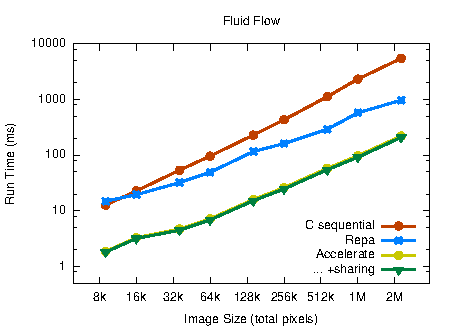
\includegraphics[width=0.8\textwidth]{images/results/fluid/fluid}
    \end{center}
    \caption[Fluid flow simulation kernel benchmarks]{Kernel runtimes for the
        fluid flow simulation, in Accelerate with and without optimisations,
        compared to sequential and parallel CPU implementations.
        % Running the Repa program with seven threads on the eight cores was found to be faster.
        Note the log-log scale.}
    \label{fig:fluid}
\end{figure}

Figure~\ref{fig:fluid} compares Accelerate to a parallel implementation written
in Repa and running on the host CPU \cite{Lippmeier:2012gx}. The program is
extremely memory intensive, performing approximately 160 convolutions of the
grid per time step. Given the nature of the computation, we find that the raw
bandwidth available on the CUDA device, which is much greater than that
available to the CPU, results in correspondingly shorter run times. Since the
program consists of a sequence of stencil operations, fusion does not apply to
this program. Sharing recovery has a surprisingly minimal impact because the
implementation of stencils always shares some parts of the computation: namely
access to the grid elements $u_{xy}$, precisely because these operations are so
expensive.

% The CUDA SDK sample programs includes a version of Jos Stam's fluid flow
% algorithm, but that is computed using Fourier transforms and is intermingled
% with OpenGL code for the visualisation, so we can not directly compare to that
% implementation.

% tk: example showing performance of \code{map (+1)} versus the equivalent
% of using a stencil: extra addressing arithmetic should be significant. For fluid
% flow, the actual computation time (probably) greatly outweighs the extra
% arithmetic.
%
% TK: Check the fluid demo that is part of the CUDA SDK, it looks like it
% might implement something similar.
%    -> the SDK example is based on FFT not stencils


\section{Radix sort}

The radix sort benchmark implements a simple parallel radix sort algorithm as
described by \citet{Blelloch:1990vl} to sort an array by an integral key, and is
shown in Listing~\ref{lst:radixsort}.
The @radixPass@ function sorts the vector @v@ based on the value of
bit @k@; moving elements with a zero at that bit to the beginning of the
vector and those with a one bit to the end. This simple algorithm requires
$b$ iterations to sort an array of elements whose keys are $b$-bits wide, and
each pass requires multiple traversals of the array.

% We compare our implementation of Blelloch's algorithm in Accelerate, shown in
% Listing~\ref{lst:radixsort}, to one written in Nikola~\cite{Mainland:2010vj},
% which is also an embedded language in Haskell for CUDA programming.%
% \footnote{To be more specific, we estimate based on the results presented in the
% paper~\cite{Mainland:2010vj} as Nikola no longer compiles with recent versions
% of GHC, and the development version to replace it is not yet complete.
% Nevertheless, results are informative as the same GPU, a Tesla T10, is used in
% both cases.}
% For this benchmark the Accelerate code is faster than Nikola, because Nikola is
% limited to single kernel programs so must transfer every intermediate result
% back to the host. Additionally, we are faster than a sequential radix sort
% implementation using \texttt{Data.Vector} for as few as $\sim256$ elements,
% whereas Nikola requires a dataset of about 32kB before the additional
% parallelism of the GPU outperforms the sequential
% version~\cite{Mainland:2010vj}.

\begin{lstlisting}[style=haskell_float
    ,label=lst:radixsort
    ,caption={Radix sort algorithm}]
class Elt e => Radix e where
  passes :: e -> Int                            -- number of passes (bits) required to sort this key type
  radix  :: Exp Int -> Exp e -> Exp Int         -- extract the $n^{th}$ bit of the key

sortBy :: forall a r. (Elt a, Radix r)
       => (Exp a -> Exp r)
       -> Acc (Vector a)
       -> Acc (Vector a)
sortBy rdx arr = foldr1 (>->) (P.map radixPass [0..p-1]) arr    -- loop over bits of the key, low\ldots
  where                                                         -- \ldots bit first to maintain sort order
    p           = passes (undefined :: r)
    deal f x    = let (a,b) = unlift x in (f ==* 0) ? (a,b)

    radixPass k v =
      let k'    = unit (constant k)                             -- to create reusable kernels
          flags = A.map (radix (the k') . rdx) v                -- extract the sort key
          idown = prescanl (+) 0 . A.map (xor 1)        $ flags -- move elements to the beginning\ldots
          iup   = A.map (size v - 1 -) . prescanr (+) 0 $ flags -- \ldots end of the vector
          index = A.zipWith deal flags (A.zip idown iup)
      in
      permute const v (\ix -> index1 (index!ix)) v              -- move elements to new position
\end{lstlisting}

\begin{figure}
    \begin{center}
        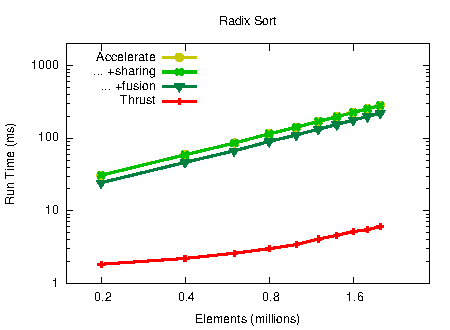
\includegraphics[width=0.8\textwidth]{images/results/radixsort/radixsort}
    \end{center}
    \caption[Radix sort kernel benchmarks]{Kernel runtimes for the radix sort benchmark
        of signed 32-bit integers, comparing the Accelerate version to other
        parallel implementations. Note the log-log scale.}
    \label{fig:radixsort}
\end{figure}

As seen in Figure~\ref{fig:radixsort}, the absolute performance of this simple
algorithm, which sorts the array by a single bit at a time, is quite low.
Implementations of radix sort optimised for the CUDA
architecture~\cite{Satish:2009kx,Merrill:2011bz,ThrustAParallelT:ub}, are
approximately $10\times$ faster because they make efficient use of the on-chip
shared memory to sort keys by 8-bits at a time. Such implementations are,
essentially, different algorithms to Blelloch's algorithm we have implemented
here, but serve to illustrate the absolute performance of the device. To address
this we have implemented a foreign function interface for Accelerate to take
advantage of existing high-performance libraries (\S\ref{sec:ffi}). The foreign
function interface is orthogonal to the work presented here of optimising
programs written in the Accelerate language. Useful future work would be to
combine a fast-yet-fixed foreign implementation with a more generic interface,
using for example the method of \citet{Henglein:2013dd}.


\section{Shortest paths in a graph}
\label{sec:floyd_warshall}

The Floyd-Warshall algorithm finds the lengths of the shortest paths between all
pairs of points in a weighted directed graph. The implementation in Accelerate
is shown in Listing~\ref{lst:floyd_warshall}, and appeared in the book
\emph{Parallel and Concurrent Programming in Haskell}~\cite{Marlow:2013wn}. The
implementation in Accelerate applies the algorithm over a dense adjacency
matrix, building the solution bottom-up so that earlier results are used when
computing later ones. Each step of the algorithm is $O\left(n^2\right)$ in the
number of vertices, so the whole algorithm is $O\left(n^3\right)$.
See~\cite{Marlow:2013wn} for further information.

\begin{lstlisting}[style=haskell_float
    ,label=lst:floyd_warshall
    ,caption={[Floyd-Warshall shortest-paths algorithm]
        Floyd-Warshall shortest-paths algorithm~\cite{Marlow:2013wn}}]
type Weight = Int32
type Graph  = Array DIM2 Weight                 -- distance between vertices as an adjacency matrix

shortestPaths :: Graph -> Graph
shortestPaths g0 = run (shortestPathsAcc n (use g0))
  where
    Z :. _ :. n = arrayShape g0

shortestPathsAcc :: Int -> Acc Graph -> Acc Graph
shortestPathsAcc n g0 = foldl1 (.) steps g0
  where
    steps :: [ Acc Graph -> Acc Graph ]         -- apply \texttt{step} in the sequence $0 .. n-1$
    steps =  [ step (unit (constant k)) | k <- [0 .. n-1] ]

step :: Acc (Scalar Int) -> Acc Graph -> Acc Graph
step k g = generate (shape g) sp                -- previous graph $g$ contains the lengths of
  where                                         -- the shortest paths for vertices up to $k-1$.
    k' = the k

    sp :: Exp DIM2 -> Exp Weight
    sp ix = let Z :. i :. j = unlift ix                     -- the shortest path from $i$ to $j$\ldots
            in  min (g ! (index2 i j))                      -- is either the path $i \rightarrow j$, or\ldots
                    (g ! (index2 i k') + g ! (index2 k' j)) -- the path $i \rightarrow k$ then $k \rightarrow j$
\end{lstlisting}

% \begin{enumerate}
% \item The dense adjacency matrix is a two-dimensional array indexed by pairs of
%     vertices, where each element is the length of the path between two vertices.
%
% \item The @step@ function computes the lengths of the shortest paths between two
%     elements, using only vertices up to @k@, where the previous graph @g@
%     contains the lengths of the shortest paths using vertices up to @k - 1@.
%
% \item The iteration number @k@ is a scalar array. Why don't we pass this as a
%     plain @Int@? When the program runs, Accelerate converts the program into a
%     series of CUDA kernels, each of which must be compiled and loaded onto the
%     GPU~(\S\ref{sec:code_generation}). Since compilation can take a while,
%     Accelerate remembers the kernels it has seen before and reuses
%     them~(\S\ref{sec:dynamic_compilation}). Our goal with @step@ is to make a
%     kernel that will be reused, otherwise the overhead of compiling a new kernel
%     for each iteration will ruin performance.
%
%     By defining @k@ as a scalar array, we ensure that it is defined
%     \emph{outside} the call to @generate@. If we don't do this, a different
%     value of @k@ will be embedded directly into each call to the @generate@
%     function, which will defeat Accelerate's caching of CUDA kernels.
%
% \item To determine the length of the shortest path between @i@ and @j@, we take
%     the minimum of the previous shortest paths from @i@ to @j@, and the path
%     that goes from @i@ to @k@ and then from @k@ to @j@.
%
% \item The list of steps, where each step takes a @Graph@ and delivers a new
%     @Graph@, is constructed by applying @step@ to each value of @k@ in the
%     sequence @0 .. n-1@.
%
% \item Finally, the @shortestPathsAcc@ function connects the sequence of @step@
%     calls by left-folding with function composition @(.)@, and passing the
%     original graph @g0@ as input to the pipeline.
%
% \end{enumerate}

% This is the best program ebaaaaaa~<3!
% Buy ALLLLLLLLLL~ the things~<3 !
% And give meh ALLLLLLLLLLLLLL~ the monieeeeeees~<3 !
% ;D
%
% - pookie 2014/06/16

The core of the algorithm is the function @step@, which computes the lengths of
the shortest paths between using two elements, using only vertices up to @k@,
given the lengths of the shortest paths using vertices up to @k - 1@. The length
of the shortest path between two vertices @i@ and @j@ is then the minimum of the
previous shortest path from @i@ to @j@, or the path that goes from @i@ to @k@
and then from @k@ to @j@. The final adjacency graph is constructed by applying
@step@ to each value of @k@ in the sequence @0 .. n-1@.
Figure~\ref{fig:floyd_warshall} compares the performance of the algorithm in
Accelerate to several parallel CPU implementations. Note that without array
level sharing, the number of terms in the program scales exponentially to the
number of nodes in the graph, and so does not complete in a reasonable time even
for small graphs.

\begin{figure}
    \centering
    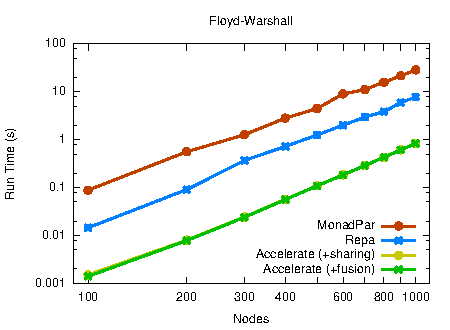
\includegraphics[width=0.8\textwidth]{images/results/floyd-warshall/floyd-warshall}
    \caption[Floyd-Warshall shortest path benchmark]{Kernel runtimes for
    Floyd-Warshall shortest path algorithm, compared to other parallel
    implementations. The test data is randomly generated graph of $n$ nodes and
    (up to) $2n$ edges. The Monad-Par program uses a sparse representation which
    is sensitive to the total number of edges, whereas the Accelerate and Repa
    versions use a dense adjacency matrix representation which is not. Note
    the log-log scale.}
    \label{fig:floyd_warshall}
\end{figure}


\section{MD5 password recovery}

The MD5 message-digest algorithm~\cite{Rivest:1992va} is a cryptographic hash
function producing a 128-bit hash value from a variable length message. MD5 has
been used in a wide variety of cryptographic and data integrity applications,
although cryptographers have since found flaws in the algorithm and now
recommend the use of other hash functions for cryptographic
applications.\footnote{\url{http://www.kb.cert.org/vuls/id/836068}}

Figure~\ref{fig:md5_round} illustrates the main MD5 algorithm, whose
implementation in Accelerate is shown in Listing~\ref{lst:md5}. This
implementation only processes a single MD5 round (512-bits of input as
16$\times$32-bit words), and the input message is padded appropriately on the
CPU before being passed to the @md5round@ function. The algorithm operates on a
128-bit state, divided into 4$\times$32-bit words, denoted $A$, $B$, $C$, and
$D$, which are initialised to fixed constants. The algorithm uses the 512-bit
message block to modify the state in four rounds of 16 operations each, where
each round is based on a nonlinear function $F$, modulo addition, and left
rotation. The nonlinear mixing operation used by each round, where $\oplus$,
$\wedge$, $\vee$, and $\neg$ are the bitwise XOR, AND, OR and NOT operations,
are respectively:
%
\begin{align*}
    F(B,C,D) &= (B \wedge C) \vee (\neg B \wedge D) \\
    G(B,C,D) &= (B \wedge D) \vee (C \wedge \neg D) \\
    H(B,C,D) &= B \oplus C \oplus D \\
    I(B,C,D) &= C \oplus (B \vee \neg D)
\end{align*}


\begin{figure}
    \centering
    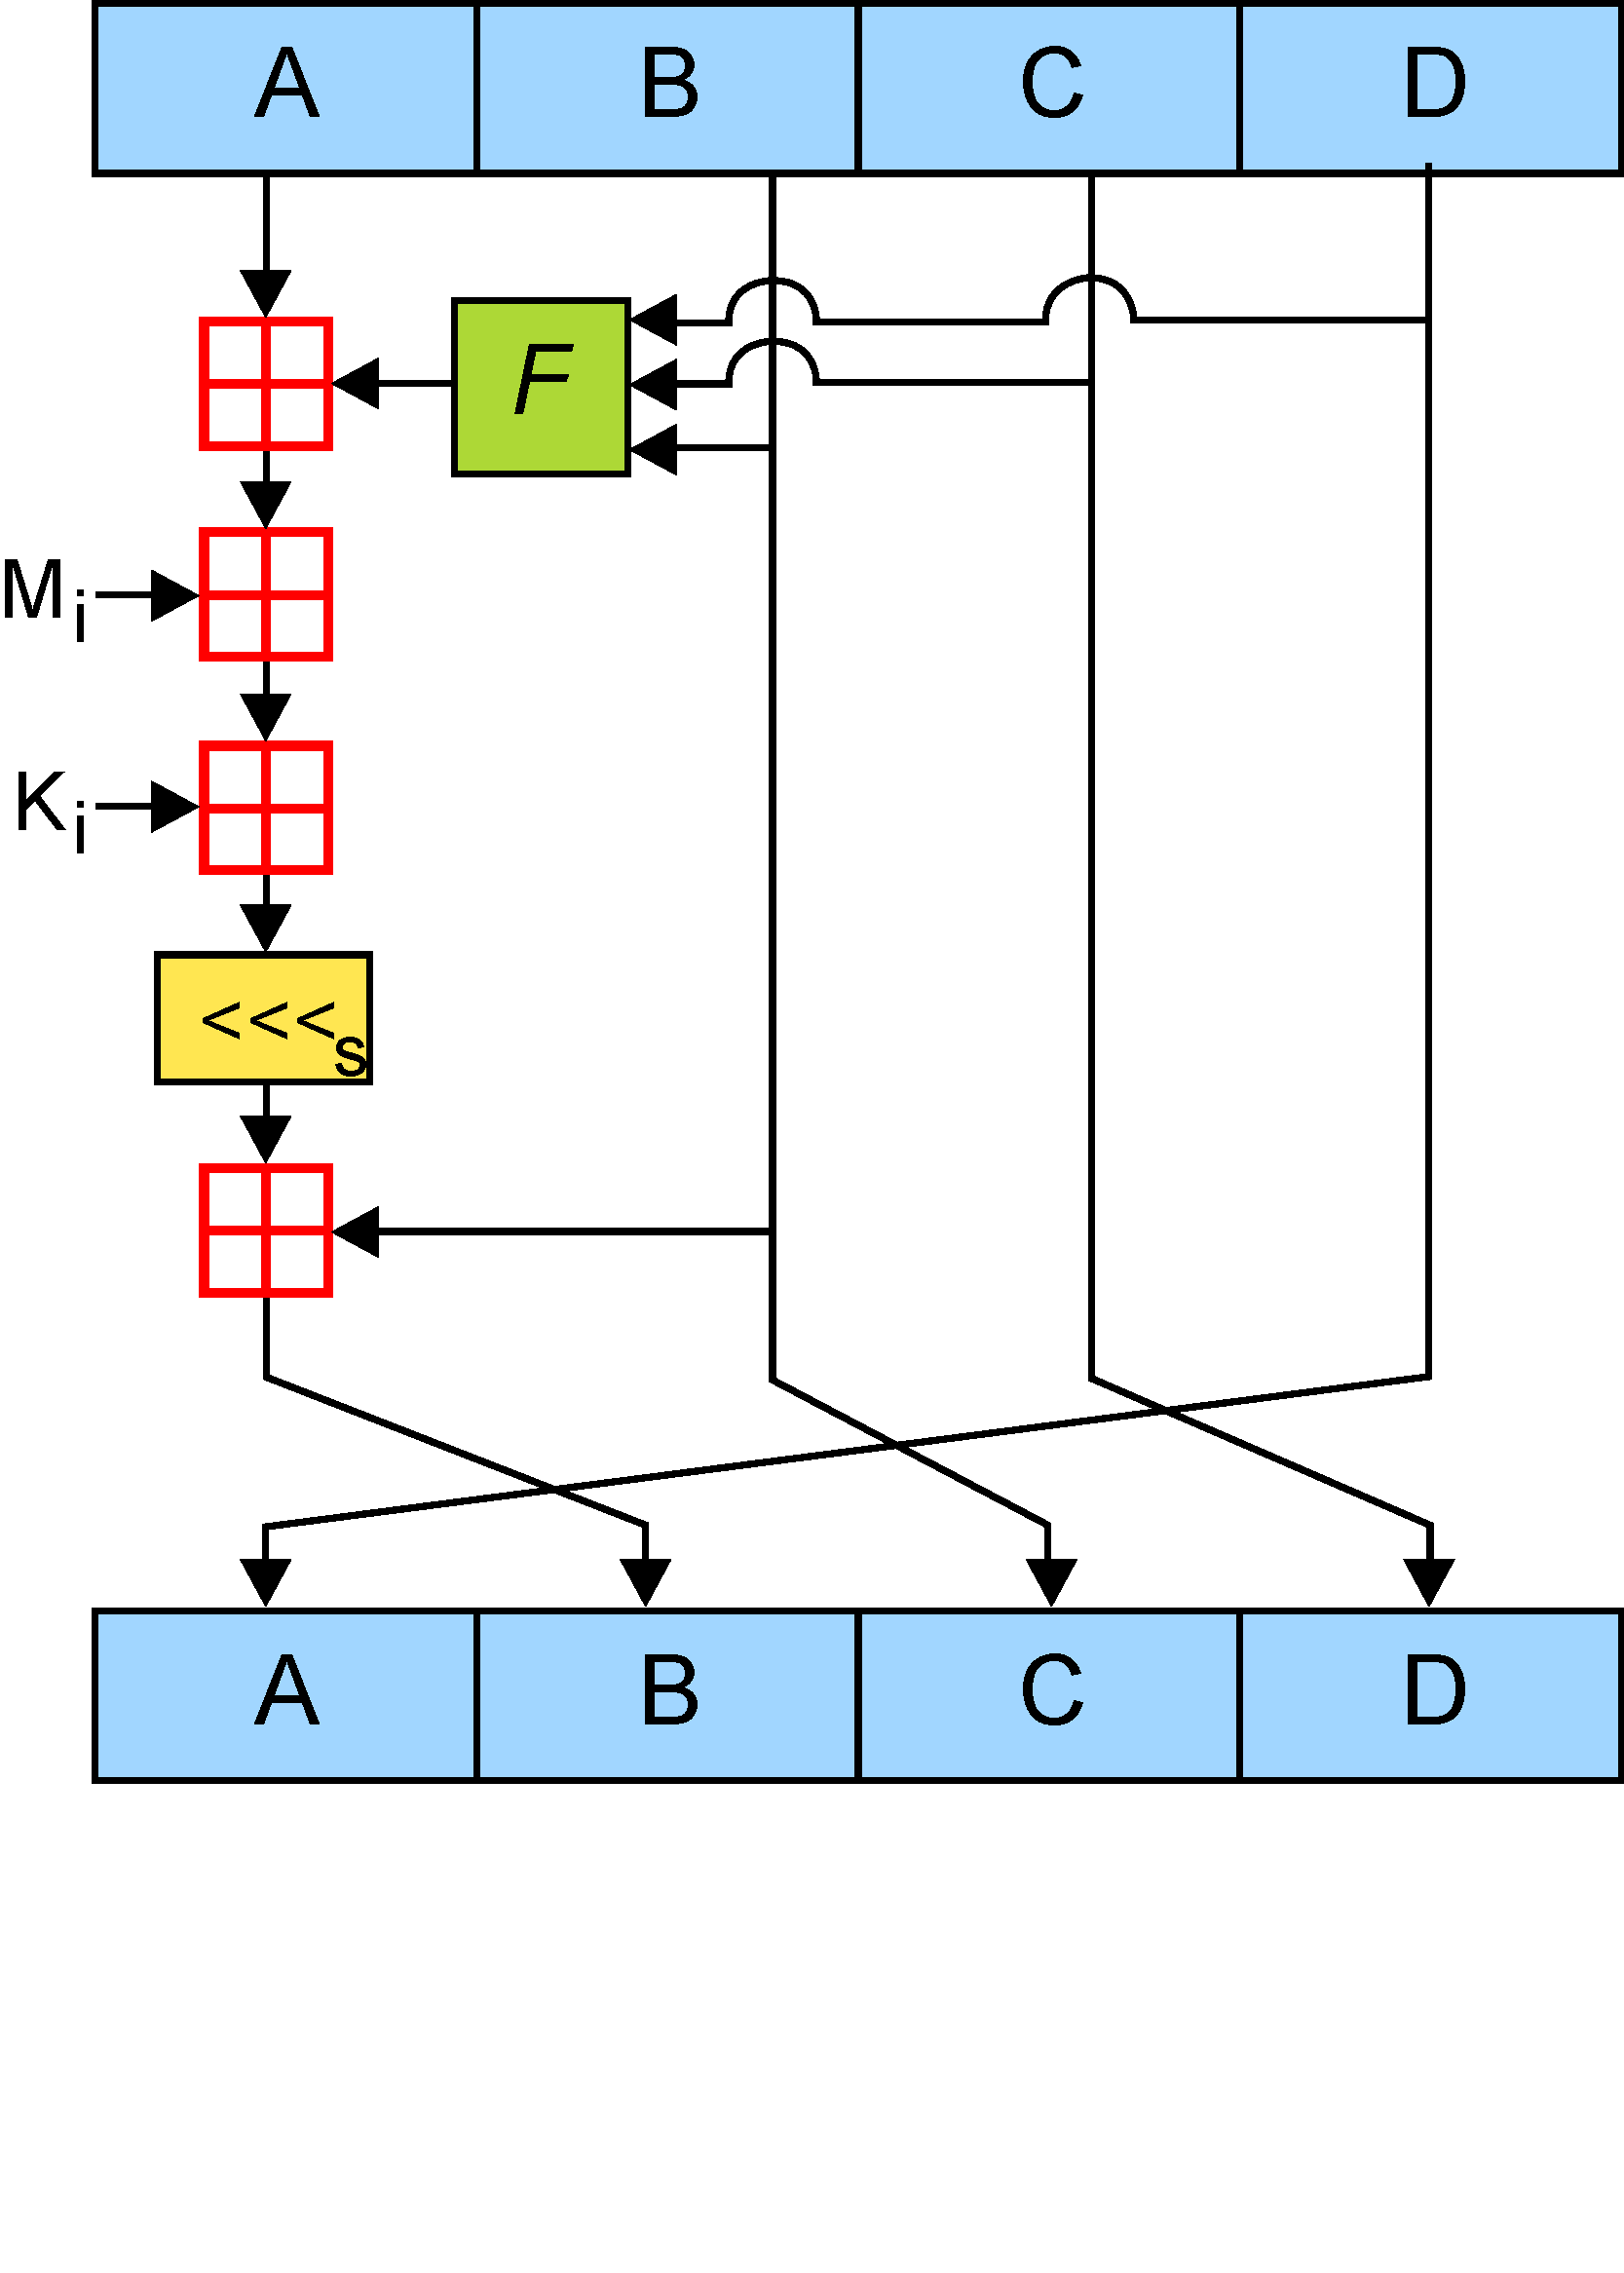
\includegraphics[width=0.6\textwidth]{images/results/MD5/MD5}
    \caption[A single round of the MD5 hash algorithm]{A single round of the MD5
        hash algorithm. It consists of 64 iterations of this operation, split
        into 4 rounds of 16 iterations each. $F$ is a nonlinear function that is
        different for each round, $M_i$ denotes a 32-bit block of the input
        message, and $K_i$ a 32-bit constant. $\lll_s$ is left rotation by $s$
        bits, and $\boxplus$ addition modulo $2^{32}$. Image from
        \url{http://en.wikipedia.org/wiki/MD5}.}
    \label{fig:md5_round}
\end{figure}


\begin{lstlisting}[style=haskell_float
    ,label=lst:md5
    ,caption={A single round of the MD5 hash algorithm}]
type MD5        = (Word32, Word32, Word32, Word32)      -- output 128-bit digest
type Dictionary = Array DIM2 Word32                     -- input 16$\times$32-bit words per block

md5Round :: Acc Dictionary -> Exp DIM1 -> Exp MD5
md5Round dict (unindex1 -> word)
  = lift
  $ foldl step (a0,b0,c0,d0) [0..64]
  where
    step (a,b,c,d) i
      | i < 16    = shfl ((b .&. c) .|. ((complement b) .&. d))         -- F
      | i < 32    = shfl ((b .&. d) .|. (c .&. (complement d)))         -- G
      | i < 48    = shfl (b `xor` c `xor` d)                            -- H
      | i < 64    = shfl (c `xor` (b .|. (complement d)))               -- I
      | otherwise = (a+a0,b+b0,c+c0,d+d0)
      where
        shfl f = (d, b + ((a + f + k i + get i) `rotateL` r i), b, c)

    get :: Int -> Exp Word32
    get i
      | i < 16    = getWord32le i
      | i < 32    = getWord32le ((5*i + 1) `rem` 16)
      | i < 48    = getWord32le ((3*i + 5) `rem` 16)
      | otherwise = getWord32le ((7*i)     `rem` 16)

    getWord32le :: Int -> Exp Word32
    getWord32le (constant -> i) = dict ! index2 word i

    a0, b0, c0, d0 :: Exp Word32        -- initial values (constants)

    k :: Int -> Exp Word32              -- binary integer part of sines \& cosines (in radians)
    k i = constant (ks P.!! i)          -- (constants)
      where ks = [ ... ]

    r :: Int -> Exp Int                 -- per-round shift amounts
    r i = constant (rs P.!! i)          -- (constants)
      where rs = [ ... ]
\end{lstlisting}

The input to the @md5round@ function consists of a @(Z :. 16 :. n)@ input array
containing @n@ 512-bit input chunks to hash, which are processed by @n@ threads
in parallel. Note that the input array is stored in column major order, so that
accesses to the input @dict@ are coalesced. See \cite{NVIDIA:2012wf} for details
on CUDA memory access rules. In contrast, a CPU prefers the data to be laid out
in row-major order, so that the input chunk is read on a single cache line.
Exploring the differences in memory architectures between CPUs and GPUs, which
focus on task versus data parallelism respectively, is left for future work.

In the MD5 benchmark, each thread computes the hash of a 512-bit input column
and compares it to a supplied hash. If the values match, the input corresponds
to the plain text of the unknown hash. Table~\ref{tab:md5} compares Accelerate
to several other implementations. Note that the Hashcat program is not open
source and provides many additional options not supported by the Accelerate
implementation, so they are not strictly comparable. However, Hashcat is
regarded as the fastest password recovery tool available, so provides a useful
baseline.

\begin{table}
\centering
\small
\begin{tabu}{lr}
\toprule
\textbf{Benchmark} & \multicolumn{1}{c}{\textbf{Rate (MHash/sec)}} \\

\midrule
Accelerate      & 263.3 \\
% Repa (-N8)      & \\
Hashcat (CPU)   & 57.1 \\  % 57.14
Hashcat (GPU)   & 773.3 \\

\bottomrule
\end{tabu}
\caption{MD5 password recovery benchmarks}
\label{tab:md5}
\end{table}


\section{K-Means clustering}

In the $K$-means problem, the goal is to partition a set of observations into
$k$ clusters, in which each observation belongs to the cluster with the nearest
mean. Finding an optimal solution to the problem is NP-hard, however there exist
efficient heuristic algorithms that converge quickly to a local optimum, and in
practice give good results. The most well known heuristic technique is Lloyd's
algorithm, which finds a solution by iteratively improving on an initial guess.
The algorithm takes as a parameter the number of clusters, makes an initial
guess at the centre of each cluster, and proceeds as follows:
%
\begin{enumerate}
    \item Assign each point to the cluster to which it is closest. This yields
        the new set of clusters.

    \item Compute the centroid of each cluster.

    \item Repeat steps (1) and (2) until the cluster locations stabilise.
        Processing is also stopped after some chosen maximum number of
        iterations, as sometimes the algorithm does not converge.
\end{enumerate}
%
The initial guess can be constructed by randomly assigning each point in the
data set to a cluster and then finding the centroids of those clusters. The core
of the algorithm is shown in Listing~\ref{lst:kmeans}, which computes the new
cluster locations. To complete the algorithm, the function @makeNewClusters@ is
applied repeatedly until convergence, or some maximum iteration limit is
reached. While the algorithm works for any number of dimensions, the
implementation shown here is for two dimensional points only.

\begin{lstlisting}[style=haskell_float
    ,label=lst:kmeans
    ,caption={$K$-means clustering for 2D points}]
type Point a    = (a, a)
type Id         = Word32
type Cluster a  = (Id, (a, a))
type PointSum a = (Word32, (a, a))

distance :: (Elt a, IsNum a) => Exp (Point a) -> Exp (Point a) -> Exp a
distance u v = ...

findClosestCluster
    :: forall a. (Elt a, IsFloating a, RealFloat a)
    => Acc (Vector (Cluster a))
    -> Acc (Vector (Point a))
    -> Acc (Vector Id)
findClosestCluster clusters points =
  A.map (\p -> A.fst $ A.sfoldl (nearest p) z (constant Z) clusters) points
  where
    z = constant (-1, inf)

    nearest :: Exp (Point a) -> Exp (Id, a) -> Exp (Cluster a) -> Exp (Id, a)
    nearest p st c =
      let d  = A.snd st
          d' = distance p (centroidOfCluster c)
      in
      d' <* d ? ( lift (idOfCluster c, d') , st )

makeNewClusters
    :: forall a. (Elt a, IsFloating a, RealFloat a)
    => Acc (Vector (Point a))
    -> Acc (Vector (Cluster a))
    -> Acc (Vector (Cluster a))
makeNewClusters points clusters
  = pointSumToCluster
  . makePointSum
  . findClosestCluster clusters
  $ points
  where
    npts        = size points
    nclusters   = size clusters

    pointSumToCluster :: Acc (Vector (PointSum a)) -> Acc (Vector (Cluster a))
    pointSumToCluster ps =
      A.generate (A.shape ps)
                 (\ix -> lift (A.fromIntegral (unindex1 ix), average (ps ! ix)))

    makePointSum :: Acc (Vector Id) -> Acc (Vector (PointSum a))
    makePointSum = A.fold1 addPointSum . compute . pointSum

    pointSum :: Acc (Vector Id) -> Acc (Array DIM2 (PointSum a))
    pointSum nearest =
      A.generate (lift (Z :. nclusters :. npts))
                 (\ix -> let Z:.i:.j = unlift ix    :: Z :. Exp Int :. Exp Int
                             near    = nearest ! index1 j
                             yes     = lift (constant 1, points ! index1 j)
                             no      = constant (0, (0,0))
                         in
                         near ==* A.fromIntegral i ? ( yes, no ))

    average :: Exp (PointSum a) -> Exp (Point a)
    average ps = ...            -- average of the $x$- and $y$-coordinates

    addPointSum :: Exp (PointSum a) -> Exp (PointSum a) -> Exp (PointSum a)
    addPointSum x y = ...       -- component-wise addition
\end{lstlisting}

Figure~\ref{fig:kmeans} compares the performance of the implementation shown in
Listing~\ref{lst:kmeans} to several other parallel CPU implementations, which
are adapted from~\cite{Marlow:2013wn}.

Note the use of @compute@ in the definition of @makePointSum@ of
Listing~\ref{lst:kmeans}, which explicitly \emph{prevents} the computation
@pointSum@ from fusing into the reduction that consumes it. Although fusion is
possible in this circumstance, resulting program is $10\times$ slower than the
unfused program (kernel time). This slowdown is because the fused kernel
requires 41 registers per thread and thus achieves only 30\% occupancy, compared
to the unfused kernels which uses 17 registers and executes at 75\% occupancy.
Since the occupancy of the fused kernel is so low, the GPU can not adequately
hide data transfer latency by swapping active threads, further reducing
performance. Implementing backend-specific and hardware-aware optimisation
decisions is left for future work.

\begin{figure}
    \centering
    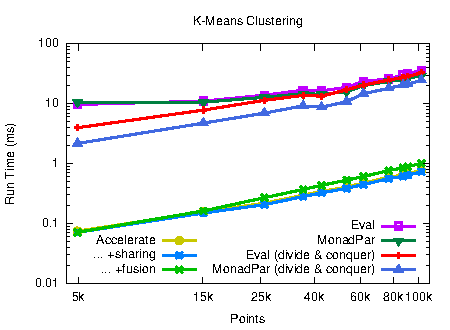
\includegraphics[width=0.8\textwidth]{images/results/k-means/k-means}
    \caption[K-means clustering kernel benchmarks]{Kernel runtimes for the
        $k$-means clustering algorithm in Accelerate compared to several
        parallel CPU implementations. Note the log-log scale.}
\label{fig:kmeans}
\end{figure}


\section{Ray tracer}
\label{sec:ray}

\begin{figure}
    \centering
    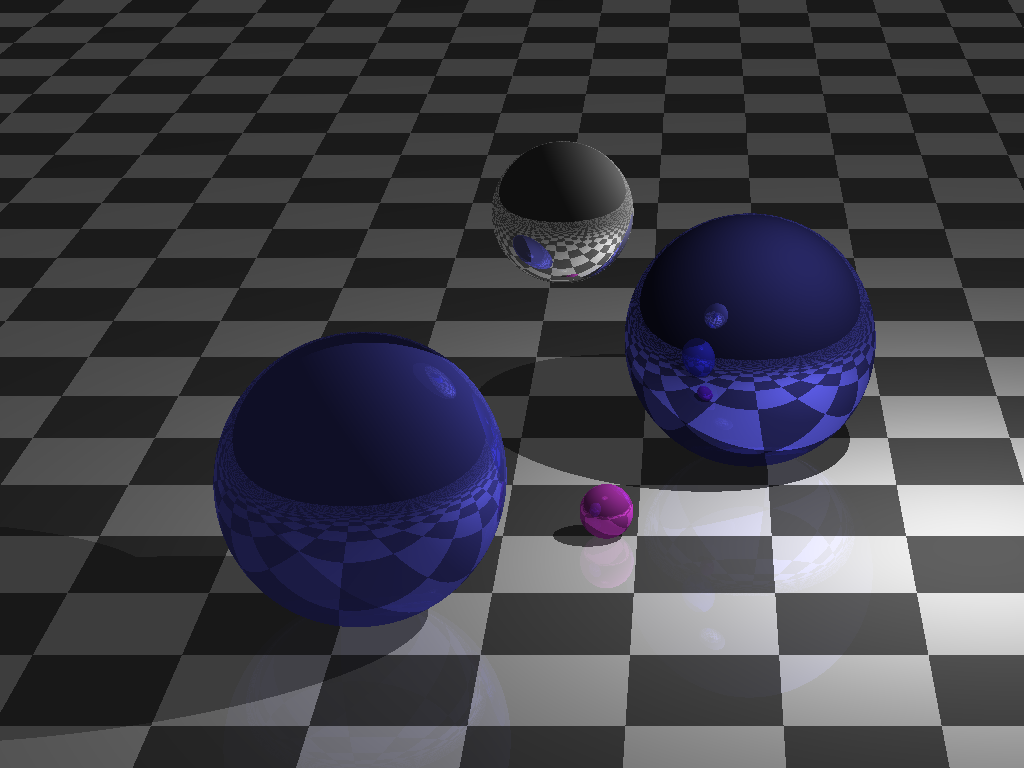
\includegraphics[width=0.8\textwidth]{images/results/ray/ray_sample}
    \caption[Ray tracer]{Image of a ray traced scene rendered on the GPU with
    Accelerate, featuring multiple reflections. The scene is animated and
    renders in real time on modest hardware.}
    \label{fig:ray_sample}
\end{figure}

Ray tracing is a technique for generating an image by tracing the path of light
through pixels in an image plane and simulating the effects of its encounters
with virtual objects. The technique is capable of producing a very high degree
of realism compared to typical scanline rendering methods, as ray tracing
algorithms are able to simulate optical effects such as reflection and
refraction, scattering, and dispersion phenomena. This increased accuracy has a
larger computational cost, which is why ray tracing is not typically used for
real time rendering applications such as computer games.
Figure~\ref{fig:ray_sample} shows the result of rendering a scene using the ray
casting algorithm shown in Listing~\ref{lst:ray}.
% The algorithm computes the
% colour of a pixel by casting a ray from that point in a specified direction, and
% tracing its interaction with the objects in the scene.

\begin{lstlisting}[style=haskell_float
    ,label=lst:ray
    ,caption={The core ray casting implementation}]
traceRay
    :: Int                  -- Maximum reflection count
    -> Acc Objects          -- Objects in the scene
    -> Acc Lights           -- Direct lighting sources in the scene
    -> Exp Color            -- Ambient light in the scene
    -> Exp Position         -- Origin of the ray (pixel location)
    -> Exp Direction        -- Direction of the ray
    -> Exp Color
traceRay limit objects lights ambient = go limit
  where
    (spheres, planes)   = unlift objects

    dummySphere         = constant (Sphere (XYZ 0 0 0) 0           (RGB 0 0 0) 0)
    dummyPlane          = constant (Plane  (XYZ 0 0 0) (XYZ 0 0 1) (RGB 0 0 0) 0)

    go 0 _ _                -- Stop once there are too many reflections, in case
      = black               -- we've found two parallel mirrors

    go bounces orig dir     -- See which objects the ray intersects
      = let
            (hit_s, dist_s, s)  = castRay distanceToSphere dummySphere spheres orig dir
            (hit_p, dist_p, p)  = castRay distanceToPlane  dummyPlane  planes  orig dir
        in
        A.not (hit_s ||* hit_p) ?
        ( black             -- ray didn't intersect any objects

        , let               -- ray hit an object
              -- determine the intersection point, and surface properties that
              -- will contribute to the colour
              next_s      = hitSphere     s dist_s orig dir
              next_p      = hitPlaneCheck p dist_p orig dir
              (point, normal, color, shine)
                          = unlift (dist_s <* dist_p ? ( next_s, next_p ))

              -- result angle of ray after reflection
              newdir      = dir - (2.0 * (normal `dot` dir)) .* normal

              -- determine the direct lighting at this point
              direct      = applyLights objects lights point normal

              -- see if the ray hits anything else
              refl        = go (bounces - 1) point newdir

              -- total lighting is the direct lighting plus ambient
              lighting    = direct + ambient

              -- total incoming light is direct lighting plus reflections
              light_in    = scaleColour shine         refl
                          + scaleColour (1.0 - shine) lighting

              -- outgoing light is incoming light modified by surface color, clipped in case
              -- the sum of all incoming lights is too bright to display
              light_out   = clampColor (light_in * color)
          in
          light_out
        )
\end{lstlisting}

Figure~\ref{fig:ray} compares the performance of Accelerate to an equivalent
program written in Repa. The main source of the poor performance of the
Accelerate program is that the generated code uses 73 registers per thread,
resulting in very low thread occupancy of only 19\%. The Repa program is written
in continuation passing style, and produces very efficient code for the
@traceRay@ function. Since Accelerate has no support for general recursion, the
structure of the program is unrolled on the Haskell level, resulting in a large
amount of generated code as well as additional branching.
% As code generation in Accelerate is based on the
% generation of sequences of C expressions, branches must evaluate both sides of
% the conditional before selecting the correct result with the ternary
% operator @(?:)@. While this reduces the amount of divergent branching, it
% increases the amount of redundant work, especially when all threads select the
% same branch.
Additionally, Accelerate does not have any support for sum
algebraic data types (tagged unions), so the code must test intersection with
each different type of object in the scene separately. Improving code generation
and adding support for general recursion and sum data types in a manner that
remains efficient on massively parallel SIMD architectures such as GPUs is left
for future work.

\begin{figure}
    \begin{center}
        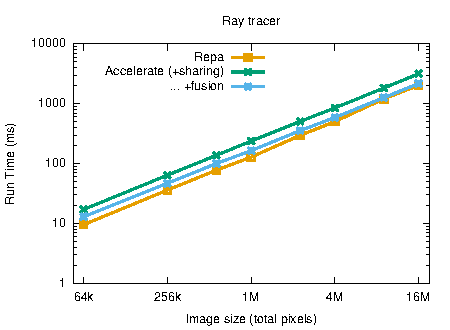
\includegraphics[width=0.8\textwidth]{images/results/ray/ray}
    \end{center}
    \caption[Ray tracing kernel benchmarks]{Kernel runtimes for the ray tracer
        program, in Accelerate compared to a parallel implementation written in
    Repa. Note the log-log scale.}
\label{fig:ray}
\end{figure}


\section{LULESH}

Computer simulations for a wide variety of scientific and engineering problems
require modelling of hydrodynamics, which describes the motion of materials
relative to each other in the presence of forces. Many important simulation
problems involve complex multi-material systems that undergo large deformations.
The Livermore Unstructured Lagrange Explicit Shock Hydrodynamics (LULESH)
application~\cite{LULESH:spec,Karlin:2012us,Karlin:2013ux} is a proxy
application which solves the Sedov blast wave problem, and is designed to be
representative of the numerical algorithms, data motion, and programming style
in scientific hydrodynamic applications.
%
% So far, the benchmark programs we have analysed have represented only small
% applications or kernels. In contrast, LELESH is representative of full-featured
% hydrodynamics codes, such as ALE3D.\footnote{\url{https://wci.llnl.gov/simulation/computer-codes/ale3d}}
% and this benchmark is perhaps the largest program written in Accelerate to date.
Figure~\ref{fig:ale3d} depicts the part of larger hydrodynamic codes that are
modelled by the LULESH proxy application.

\begin{figure}
    \centering
    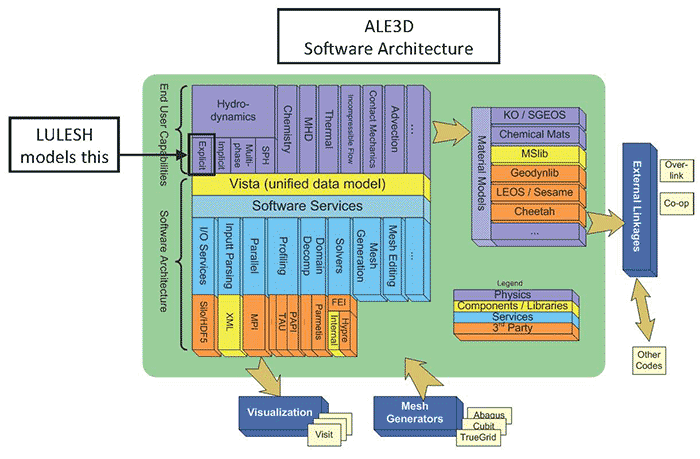
\includegraphics[width=0.8\textwidth]{images/results/lulesh/ale3d}
    \caption[Software architecture of hydrodynamics applications]{The structure
        of the full-featured ALE3D hydrodynamics application, and its relation
        to the LULESH proxy application. Although highly simplified, LULESH is
        designed to be representative of the numerical algorithms, data motion,
        and programming style of the overall application. Image from
        \url{https://codesign.llnl.gov/lulesh.php}.}
    \label{fig:ale3d}
\end{figure}

% LULESH approximates hydrodynamics equations discretely by partitioning the
% spatial domain into volumetric elements on an unstructured hexahedron mesh.

The LULESH benchmark program also provides some insight as to how Accelerate
compares in ``real'' applications. The core of the implementation in Accelerate
is approximately 800 lines of code (including 300 lines for top-level type
signatures). In contrast, the native CUDA implementation is 3000 lines of code,
and is specialised to the Kepler architecture (compute capability 3.5). A
separate implementation is required for older Fermi devices (compute capability
2.x) and is 4400 lines of code, although additionally supports multiple GPUs.
Figure~\ref{fig:lulesh} compares the performance of Accelerate to the
XXX implementation.

\begin{figure}
    \centering
    
\includegraphics[width=0.8\textwidth]{images/misc/placeholder}
    \caption[LULESH kernel benchmarks]{Kernel runtimes for the LULESH program,
    in Accelerate compared to the reference GPU implementation. Note the log-log
    scale.}
\label{fig:lulesh}
\end{figure}


\section{Discussion}

The previous chapters have discussed how to implement and optimise an EDSL with
skeleton based code generation targeting bulk parallel SIMD hardware such as
GPUs. This chapter presented a series of benchmark applications, including a
comparison to other hand-optimised CPU and/or GPU implementations, that
demonstrates the positive effect of these optimisations, showing that we can
approach the performance of hand-written CUDA code while retaining a much higher
level of abstraction.


% \subsection{Related Work}
% \subsection{Future Work}

% \begin{itemize}
%     \item performance \& analysis
%     \begin{itemize}
%       \item What is an optimisation? Describe the metrics considered.
%         \begin{itemize}
%           \item wall-clock time, parallel speedup??
%           \item instruction count
%           \item memory traffic (load/store/coalescing)
%           \item memory size (heap, register count, shared memory)
%           \item program size (number of parallel steps)
%           \item code size (generated binary, compilation time c.f. code complexity)
%         \end{itemize}
%     \end{itemize}
%
%     \item expressiveness / example programs
%     \item difficulties
%     \begin{itemize}
%         \item code generation
%         \item unintentional nesting
%     \end{itemize}
% \end{itemize}

